\chapter{Lab 2: QMC Basics}
\label{chap:lab_qmc_basics}



\section{Topics covered in this Lab}
This lab focuses on the basics of performing quality QMC calculations.  As an example participants test an oxygen pseudopotential within DMC by calculating atomic and dimer properties, a common step prior to production runs.  Topics covered include:
\begin{itemize}
  \item{converting pseudopotentials into QMCPACK's FSATOM format}
  \item{generating orbitals with Quantum ESPRESSO}
  \item{converting orbitals into QMCPACK's ESHDF format with pw2qmcpack}
  \item{optimizing Jastrow factors with QMCPACK}
  \item{removing DMC timestep error via extrapolation}
  \item{automating QMC workflows with Nexus}
  \item{testing pseudopotentials for accuracy}
  \hide{
  \item{(optional) running QMCPACK for a general system of interest}
  }
\end{itemize}

\section{Lab outline}
\begin{enumerate}
  \item{download and conversion of oxygen atom pseudopotential}
  \item{DMC timestep study of the neutral oxygen atom}
  \begin{enumerate}
    \item{DFT orbital generation with Quantum ESPRESSO}
    \item{orbital conversion with \texttt{pw2qmcpack.x}}
    \item{optimization of Jastrow correlation factor with QMCPACK}
    \item{DMC run with multiple timesteps}
  \end{enumerate}
  \item{DMC timestep study of the first ionization potential of oxygen}
  \begin{enumerate}
    \item{repetition of a-d above for ionized oxygen atom}
  \end{enumerate}
  \item{automated DMC calculations of the oxygen dimer binding curve}
\end{enumerate}


\section{Lab directories and files}
\footnotesize
\begin{verbatim}%
labs/lab2_qmc_basics/
│
├── oxygen_atom           - oxygen atom calculations 
│   ├── O.q0.dft.in          - Quantum ESPRESSO input for DFT run
│   ├── O.q0.p2q.in          - pw2qmcpack.x input for orbital conversion run
│   ├── O.q0.opt.in.xml      - QMCPACK input for Jastrow optimization run
│   ├── O.q0.dmc.in.xml      - QMCPACK input file for neutral O DMC
│   ├── ip_conv.py           - tool to fit oxygen IP vs timestep
│   └── reference            - directory w/ completed runs
│
├── oxygen_dimer          - oxygen dimer calculations
│   ├── dimer_fit.py         - tool to fit dimer binding curve
│   ├── O_dimer.py           - automation script for dimer calculations
│   ├── pseudopotentials     - directory for pseudopotentials
│   └── reference            - directory w/ completed runs
│
└── your_system           - performing calculations for an arbitrary system (yours)
    ├── example.py           - example nexus file for periodic diamond
    ├── pseudopotentials     - directory containing C pseudopotentials
    └── reference            - directory w/ completed runs
\end{verbatim}
\normalsize

\section{Obtaining and converting a pseudopotential for oxygen}
\label{sec:lqb_pseudo}
First enter the \texttt{oxygen\_atom} directory:
\begin{shade}
cd labs/lab2_qmc_basics/oxygen_atom/
\end{shade}
\noindent
Throughout the rest of the lab, locations will be specified with respect to \texttt{labs/lab2\_qmc\_basics} (e.g. \texttt{oxygen\_atom}).

We will use a potential from the Burkatzki-Filippi-Dolg pseudopotential database.  
Although the full database is available in QMCPACK distribution (\texttt{trunk/pseudopotentials/BFD/}), 
we use a BFD pseudopotential to illustrate the process of converting and testing an 
external potential for use with QMCPACK.   To obtain the pseudopotential, go to 
\href{http://www.burkatzki.com/pseudos/index.2.html}{http://www.burkatzki.com/pseudos/index.2.html}
and click on the ``Select Pseudopotential'' button.  Next click on oxygen in the 
periodic table.  Click on the empty circle next to ``V5Z'' (a large gaussian 
basis set) and click on ``Next''.  Select the Gamess format and click on 
``Retrive Potential''.  Helpful information about the pseudopotential will be 
displayed.  The desired portion is at the bottom (the last 7 lines).  Copy 
this text into the editor of your choice (e.g. \texttt{emacs} or \texttt{vi}) 
and save it as \texttt{O.BFD.gamess} 
(be sure to include a newline at the end of the file).  To transform the 
pseudopotential into the FSATOM XML format used by QMCPACK, use the \texttt{ppconvert} 
tool:

\noindent
\ifws
\begin{shade}
ppconvert --gamess_pot O.BFD.gamess --s_ref "1s(2)2p(4)" \
 --p_ref "1s(2)2p(4)" --d_ref "1s(2)2p(4)" --xml O.BFD.xml
\end{shade}
\else
\begin{shade}
jobrun_vesta ppconvert --gamess_pot O.BFD.gamess --s_ref "1s(2)2p(4)" \
 --p_ref "1s(2)2p(4)" --d_ref "1s(2)2p(4)" --xml O.BFD.xml
\end{shade}
\fi

\noindent
Observe the notation used to describe the reference valence configuration for this helium-core PP: \texttt{1s(2)2p(4)}.  The \texttt{ppconvert} tool uses the following convention for the valence states: the first $s$ state is labeled \texttt{1s} (\texttt{1s}, \texttt{2s}, \texttt{3s}, \ldots), the first $p$ state is labeled \texttt{2p} (\texttt{2p}, \texttt{3p}, \ldots), the first $d$ state is labeled \texttt{3d} (\texttt{3d}, \texttt{4d}, \ldots). Copy the resulting xml file into the \texttt{oxygen\_atom} directory.

Note: the command to convert the PP into QM Espresso's UPF format is similar (both formats are required):

\noindent
\ifws
\begin{shade}
ppconvert --gamess_pot O.BFD.gamess --s_ref "1s(2)2p(4)" \
 --p_ref "1s(2)2p(4)" --d_ref "1s(2)2p(4)" --log_grid --upf O.BFD.upf
\end{shade}
\else
\begin{shade}
jobrun_vesta ppconvert --gamess_pot O.BFD.gamess --s_ref "1s(2)2p(4)" \
 --p_ref "1s(2)2p(4)" --d_ref "1s(2)2p(4)" --log_grid --upf O.BFD.upf
\end{shade}
\noindent
\fi

For reference, the text of \texttt{O.BFD.gamess} should be:
\begin{lstlisting}
O-QMC GEN 2 1
3
6.00000000 1 9.29793903
55.78763416 3 8.86492204
-38.81978498 2 8.62925665
1
38.41914135 2 8.71924452

\end{lstlisting}
\noindent
The full QMCPACK pseudopotential is also included in \texttt{oxygen\_atom/reference/O.BFD.*}.


\section{DFT with Quantum ESPRESSO to obtain the orbital part of the wavefunction}
\label{sec:lqb_dft}
With the pseudopotential in hand, the next step toward a QMC calculation is to obtain the Fermionic part of the wavefunction, in this case a single Slater determinant constructed from DFT-LDA orbitals for a neutral oxygen atom.  If you had trouble with the pseudopotential conversion step, pre-converted pseudopotential files are located in the \texttt{oxygen\_atom/reference} directory.  

Quantum ESPRESSO input for the DFT-LDA ground state of the neutral oxygen atom can be found in \texttt{O.q0.dft.in} and also listing \ref{lst:O_q0_dft} below.  Setting \texttt{wf\_collect=.true.} instructs Quantum Espresso to write the orbitals to disk at the end of the run. Option \texttt{wf\_collect=.true.} may be a potential problem in large simulations, it is recommended to avoid it and use the converter pw2qmcpack in parallel, see details in Sec.~\ref{sec:pw2qmcpack}. Note that the plane-wave energy cutoff has been set to a reasonable value of 300 Ry here (\texttt{ecutwfc=300}).  This value depends on the pseudopotentials used, and in general should be selected by running DFT$\rightarrow$(orbital conversion)$\rightarrow$VMC with increasing energy cutoffs until the lowest VMC total energy and variance is reached.

\begin{lstlisting}[caption={Quantum ESPRESSO input file for the neutral oxygen atom (\texttt{O.q0.dft.in})\label{lst:O_q0_dft}}]
&CONTROL
   calculation       = 'scf'
   restart_mode      = 'from_scratch'
   prefix            = 'O.q0'
   outdir            = './'
   pseudo_dir        = './'
   disk_io           = 'low'
   wf_collect        = .true.
/

&SYSTEM
   celldm(1)         = 1.0
   ibrav             = 0
   nat               = 1
   ntyp              = 1
   nspin             = 2
   tot_charge        = 0
   tot_magnetization = 2
   input_dft         = 'lda'
   ecutwfc           = 300
   ecutrho           = 1200
   nosym             = .true.
   occupations       = 'smearing'
   smearing          = 'fermi-dirac'
   degauss           = 0.0001
/

&ELECTRONS
   diagonalization   = 'david'
   mixing_mode       = 'plain'
   mixing_beta       = 0.7
   conv_thr          = 1e-08
   electron_maxstep  = 1000
/


ATOMIC_SPECIES 
   O  15.999 O.BFD.upf

ATOMIC_POSITIONS alat
   O     9.44863067       9.44863161       9.44863255

K_POINTS automatic
   1 1 1  0 0 0 

CELL_PARAMETERS cubic
        18.89726133       0.00000000       0.00000000 
         0.00000000      18.89726133       0.00000000 
         0.00000000       0.00000000      18.89726133
\end{lstlisting}

Run Quantum ESPRESSO by typing 
\ifws
\begin{shade}
mpirun -np 4 pw.x -input O.q0.dft.in >&O.q0.dft.out&
\end{shade}
\else
\begin{shade}
jobrun_vesta pw.x O.q0.dft.in
\end{shade}
\fi

The DFT run should take a few minutes to complete.  If desired, you can track the progress of the DFT run by typing ``\ifws\verb|tail -f O.q0.dft.out|\else\verb|tail -f O.q0.dft.output|\fi''. Once finished, you should check the LDA total energy in \texttt{\labsw{O.q0.dft.out}{O.q0.dft.output}} by typing ``\ifws\verb|grep '!  ' O.q0.dft.out|\else\verb|grep '!  ' O.q0.dft.output|\fi''.  The result should be close to
\begin{shade}
!    total energy              =     -31.57553905 Ry
\end{shade} 
% both of the numbers below are for 200 Ry (too small as it turns out)
% 10 Angstrom cell
%!    total energy              =     -31.56729415 Ry
% 15 Angstrom cell
%!    total energy              =     -31.56730213 Ry



The orbitals have been written in a format native to Quantum ESPRESSO in the \texttt{O.q0.save} directory.  We will convert them into the ESHDF format expected by QMCPACK by using the \texttt{pw2qmcpack.x} tool.  The input for \texttt{pw2qmcpack.x} can be found in the file \texttt{O.q0.p2q.in} and also in listing \ref{lst:O_q0_p2q} below. 

\begin{lstlisting}[caption={\texttt{pw2qmcpack.x} input file for orbital conversion (\texttt{O.q0.p2q.in})\label{lst:O_q0_p2q}}]
&inputpp
  prefix     = 'O.q0'
  outdir     = './'
  write_psir = .false.
/
\end{lstlisting}

Perform the orbital conversion now by typing the following:
\ifws
\begin{shade}
mpirun -np 1 pw2qmcpack.x<O.q0.p2q.in>&O.q0.p2q.out&
\end{shade}
\else
\begin{shade}
jobrun_vesta pw2qmcpack.x O.q0.p2q.in
\end{shade}
\fi
\noindent
Upon completion of the run, a new file should be present containing the orbitals for QMCPACK: \texttt{O.q0.pwscf.h5}.  Template XML files for particle (\texttt{O.q0.ptcl.xml}) and wavefunction (\texttt{O.q0.wfs.xml}) inputs to QMCPACK should also be present.  


\section{Optimization with QMCPACK to obtain the correlated part of the wavefunction}\label{sec:optimization_walkthrough}
The wavefunction we have obtained to this point corresponds to a non-interacting Hamiltonian.  Once the Coulomb pair potential is switched on between particles, it is known analytically that the exact wavefunction has cusps whenever two particles meet spatially and in general the electrons become correlated.  This is represented in the wavefunction by introducing a Jastrow factor containing at least pair correlations
\begin{align}
  &\Psi_{Slater-Jastrow}=e^{-J}\Psi_{Slater} \\
  &J = \sum_{\sigma\sigma'}\sum_{i<j}u^{\sigma\sigma'}_2(|r_i-r_j|) + \sum_\sigma\sum_{iI}u^{\sigma I}_1(|r_i-r_I|)
\end{align}
Here $\sigma$ is a spin variable while $r_i$ and $r_I$ represent electron and ion coordinates, respectively.  The introduction of $J$ into the wavefunction is similar to F12 methods in quantum chemistry, though it has been present in essentially all QMC studies since the first applications the method (circa 1965).

How are the functions $u_2^{\sigma\sigma'}$ and $u_1^{\sigma}$ obtained?  Generally, they are approximated by analytical functions with several unknown parameters that are determined by minimizing the energy or variance directly within VMC.  This is effective because the energy and variance reach a global minimum only for the true ground state wavefunction ($\textrm{Energy}=E\equiv\expval{\Psi}{\hat{H}}{\Psi}$, $\textrm{Variance}=V\equiv\expval{\Psi}{(\hat{H}-E)^2}{\Psi}$).  For this exercise, we will focus on minimizing the variance.

% background on the wavefunction should be covered elsewhere in the manual
%   perhaps replace this with just the figure and a couple of brief comments 
\hide{
\subsubsection{Background on trial wavefunction and optimization}\label{sec:opt_background}
The trial wavefunction used to describe the neutral oxygen atom is of the 
standard Slater-Jastrow form:
\begin{align}  
  \Psi_T = e^{-(J_1+J_2)}D^\uparrow(\{\phi_u^\uparrow\}_{u=1}^{N^\uparrow})D^\downarrow(\{\phi_d^\downarrow\}_{d=1}^{N^\uparrow})
\end{align}
The orbitals forming the spin-restricted Slater determinants 
($D^\uparrow/D^\downarrow$) are obtained from DFT or Hartree-Fock (\emph{e.g.} via Quantum ESPRESSO) 
and are fixed.  The ground state of the (pseudo) oxygen atom is spin polarized 
with $N^{\uparrow}=4$ and $N^{\downarrow}=2$.  

The part of the wavefunction we will be optimizing is the Jastrow factor 
($e^{-(J_1+J_2)}$), which in this case includes one- (electron-ion) and two- 
(electron-electron) body correlation functions.  The Jastrow factor is symmetric 
under same-spin electron exchange and does not affect the DMC fixed node 
approximation.  Optimization of the Jastrow factor does, however, improve the 
efficiency of the DMC calculation and reduces additional approximations due to 
non-local pseudopotentials (locality approximation, T-moves).  Note that a three-body 
term ($J_3$) is also available and is often necessary when using pseudopotentials 
for transition metal species or when high accuracy is desired for molecules.  


\begin{figure}
\begin{center}
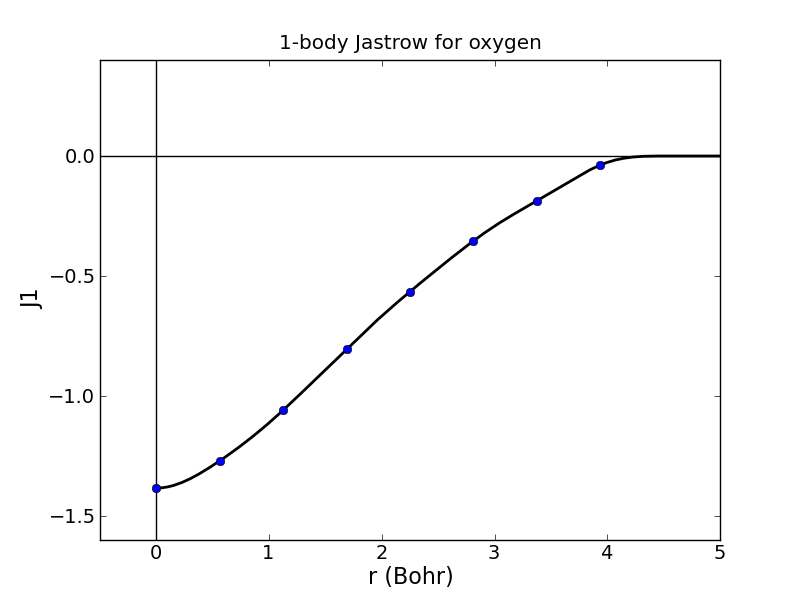
\includegraphics[trim = 0mm 0mm 0mm 0mm, clip,width=0.75\columnwidth]{./figures/lab_qmc_basics_J1.png}
\end{center}
\caption{Optimized $U_1$ function for 1-body Jastrow factor of an oxygen atom.
\label{fig:u1_spline}
}
\end{figure}

The explicit form of the one-body Jastrow factor we will be using is
\begin{align}\label{eq:J1}
  J_1 = \sum_{e=1}^{N^\uparrow+N^\downarrow}U_1^{\uparrow/\downarrow}(|r_e-r_O|)
\end{align}
where $r_e$ refers to the electron positions and $r_O$ is 
the position of the oxygen ion.  The $U_1^{\uparrow/\downarrow}$ term is a 
one-dimensional radial function represented with piecewise continuous cubic 
polynomials (B-splines).  The adjustable parameters to be optimized are the 
``knots'' of the B-splines which are simply the values of the $U_1$ function at 
uniformly spaced grid points (See fig. \ref{fig:u1_spline} for an example of a $U_1$ 
spline function with 8 knots).  

The two-body Jastrow factor is spin resolved ($r^\uparrow/r^\downarrow$ are up/down electron positions):
\begin{align}\label{eq:J2}
  J_2 = \sum_{u<u'}U_2^{\uparrow\uparrow/\downarrow\downarrow}(|r_u^\uparrow-r_{u'}^\uparrow|) + \sum_{d<d'}U_2^{\uparrow\uparrow/\downarrow\downarrow}(|r_d^\downarrow-r_{d'}^\downarrow|) + \sum_{u,d} U_2^{\uparrow\downarrow}(|r_u^\uparrow-r_d^\downarrow|)
\end{align}
For an atom, Pad\'{e} functions are appropriate for $U_2^{\uparrow\uparrow/\downarrow\downarrow}$ and $U_2^{\uparrow\downarrow}$:
\begin{align}
  U_2(r) = \frac{Ar}{1+Br}
\end{align}
Only $B^{\uparrow\uparrow/\downarrow\downarrow}$ and $B^{\uparrow\downarrow}$ are adjustable since the $A$ parameters are fixed by the electron-electron cusp conditions.

Wavefunction optimization essentially relies on two inequalities regarding energy and variance:
\begin{align}
  E_T(P) &= \frac{\expvalh{\Psi_T(P)}{H}{\Psi_T(P)}}{\overlap{\Psi_T(P)}{\Psi_T(P)}} \ge E_0 \\
  V_T(P) &= \frac{\expval{\Psi_T(P)}{\hat{H}^2}{\Psi_T(P)}}{\overlap{\Psi_T(P)}{\Psi_T(P)}} - \left(\frac{\expval{\Psi_T(P)}{H}{\Psi_T(P)}}{\overlap{\Psi_T(P)}{\Psi_T(P)}}\right)^2 \ge 0   
\end{align}
Here $E_0$ is the ground state energy, $E_T(P)$ is the trial energy, $V_T(P)$ is the trial variance, and $P$ denotes the set of adjustable parameters in the trial wavefunction.  Equality is reached only for the true ground state wavefunction and so the trial wavefunction can be improved by attempting to minimize a chosen cost function: 
\begin{align}
  C(P) = \alpha E_T(P) + (1-\alpha) V_T(P).
\end{align}  
Iterative varational Monte Carlo methods have been developed to handle the non-linear optimization problem $\min\limits_P C(P)$.  We will be using the linearized optimization method of Umrigar, \emph{et al.} (PRL \textbf{98} 110201 (2007)).  Let us try this now with QMCPACK.
}

First, we need to update the template particle and wavefunction information in \texttt{O.q0.ptcl.xml} and \texttt{O.q0.wfs.xml}.  We want to simulate the O atom in open boundary conditions (the default is periodic).  To do this open \texttt{O.q0.ptcl.xml} with your favorite text editor (e.g. \texttt{emacs} or \texttt{vi}) and replace
\begin{lstlisting}[language=xml]
<parameter name="bconds">
   p p p
</parameter>
<parameter name="LR_dim_cutoff">
   15
</parameter>
\end{lstlisting}
with
\begin{lstlisting}[language=xml]
<parameter name="bconds">
   n n n 
</parameter>
\end{lstlisting}

Next we will select Jastrow factors appropriate for an atom.  In open boundary conditions, the B-spline Jastrow correlation functions should cut off to zero at some distance away from the atom.  Open \texttt{O.q0.wfs.xml} and add the following cutoffs (\texttt{rcut} in Bohr radii) to the correlation factors:
\begin{lstlisting}
...
<correlation speciesA="u" speciesB="u" size="8" rcut="10.0">
...
<correlation speciesA="u" speciesB="d" size="8" rcut="10.0">
...
<correlation elementType="O" size="8" rcut="5.0">
...
\end{lstlisting}
\noindent
These terms correspond to $u_2^{\uparrow\uparrow}/u_2^{\downarrow\downarrow}$, $u_2^{\uparrow\downarrow}$, and $u_1^{\uparrow O}/u_1^{\downarrow O}$, respectively.  In each case, the correlation function ($u_*$) is represented by piecewise continuous cubic B-splines.  Each correlation function has eight parameters which are just the values of $u$ on a uniformly spaced grid up to \texttt{rcut}.  Initially the parameters (\texttt{coefficients}) are set to zero:
\begin{lstlisting}
<correlation speciesA="u" speciesB="u" size="8" rcut="10.0">
  <coefficients id="uu" type="Array">
     0.0 0.0 0.0 0.0 0.0 0.0 0.0 0.0
  </coefficients>
</correlation>
\end{lstlisting}

Finally, we need to assemble particle, wavefunction, and pseudopotential information into the main QMCPACK input file (\texttt{O.q0.opt.in.xml}) and specify inputs for the Jastrow optimization process.  Open \texttt{O.q0.opt.in.xml} and write in the location of the particle, wavefunction, and pseudopotential files (``\texttt{<!-- ... -->}'' are comments):
\begin{lstlisting}
...
<!-- include simulationcell and particle information from pw2qmcpqack -->
<include href="O.q0.ptcl.xml"/>
...
<!-- include wavefunction information from pw2qmcpqack -->
<include href="O.q0.wfs.xml"/>
...
<!-- O pseudopotential read from "O.BFD.xml" -->
<pseudo elementType="O" href="O.BFD.xml"/>
...
\end{lstlisting}
\noindent
The relevant portion of the input describing the linear optimization process is
\begin{lstlisting}
<loop max="MAX">  
  <qmc method="linear" move="pbyp" checkpoint="-1">
    <cost name="energy"              >  ECOST    </cost>
    <cost name="unreweightedvariance">  UVCOST   </cost>
    <cost name="reweightedvariance"  >  RVCOST   </cost>
    <parameter name="timestep"       >  TS       </parameter>
    <parameter name="samples"        >  SAMPLES  </parameter>
    <parameter name="warmupSteps"    >  50       </parameter>
    <parameter name="blocks"         >  200      </parameter>
    <parameter name="subSteps"       >  1        </parameter>
    <parameter name="nonlocalpp"     >  yes      </parameter>
    <parameter name="useBuffer"      >  yes      </parameter>
    ...
  </qmc>
</loop>
\end{lstlisting}
\noindent
An explanation of each input variable can be found below.  The remaining variables control specialized internal details of the linear optimization algorithm.  The meaning of these inputs is beyond the scope of this lab and reasonable results are often obtained keeping these values fixed. 
\begin{description}
  \item[energy] Fraction of trial energy in the cost function.
  \item[unreweightedvariance] Fraction of unreweighted trial variance in the cost function.  Neglecting the weights can be more robust.
  \item[reweightedvariance] Fraction of trial variance (including the full weights) in the cost function.  
  \item[timestep] Timestep of the VMC random walk, determines spatial distance moved by each electron during MC steps.  Should be chosen such that the acceptance ratio of MC moves is around 50\% (30-70\% is often acceptable).  Reasonable values are often between 0.2 and 0.6 $\textrm{Ha}^{-1}$.
  \item[samples] Total number of MC samples collected for optimization, determines statistical error bar of cost function.  Often efficient to start with a modest number of samples (50k) and then increase as needed.  More samples may be required if the wavefunction contains a large number of variational parameters.  MUST be be a multiple of the number of threads/cores \labsw{}{(use multiples of 512 on Vesta)}.
  \item[warmupSteps]  Number of MC steps discarded as a warmup or equilibration period of the random walk.  If this is too small, it will bias the optimization procedure.
  \item[blocks]  Number of average energy values written to output files.  Should be greater than 200 for meaningful statistical analysis of output data (\emph{e.g.} via \texttt{qmca}).
  \item[subSteps] Number of MC steps in between energy evaluations.  Each energy evaluation is expensive so taking a few steps to decorrelate between measurements can be more efficient.  Will be less efficient with many substeps.
  \item[nonlocalpp,useBuffer] If \texttt{nonlocalpp="no"}, then nonlocal part of the pseudopotential is not included when computing the cost function.  If \texttt{useBuffer="yes"}, then temporary data is stored to speed up nonlocal pseudopotential evaluation at the expense of memory consumption.  
  \item[loop max] Number of times to repeat the optimization.  Using the resulting wavefunction from the previous optimization in the next one improves the results.  Typical choices range between 8 and 16.   
\end{description}
The cost function defines the quantity to be minimized during optimization. The three components of the cost function, energy, unreweighted variance, and reweighted variance should sum to one.  Dedicating 100\% of the cost function to unreweighted variance is often a good choice.  Another common choice is to try 90/10 or 80/20 mixtures of reweighted variance and energy.  Using 100\% energy minimization is desirable for reducing DMC pseudopotential localization errors, but the optimization process is less stable and should only be attempted after performing several cycles of e.g. variance minimization first (the entire \texttt{loop} section can be duplicated with a different cost function each time).

Replace \texttt{MAX}, \texttt{EVCOST}, \texttt{UVCOST}, \texttt{RVCOST}, \texttt{TS}, and \texttt{SAMPLES} in the \texttt{loop} with appropriate starting values in the \texttt{O.q0.opt.in.xml} input file.  Perform the optimization run by typing
\ifws
\begin{shade}
mpirun -np 4 qmcpack O.q0.opt.in.xml >&O.q0.opt.out&
\end{shade}
\else
\begin{shade}
jobrun_vesta qmcpack O.q0.opt.in.xml
\end{shade}
\fi
\noindent
The run should only take a few minutes for reasonable values of loop \texttt{max} and \texttt{samples}.  

Log file output will appear in \labsw{\texttt{O.q0.opt.out}}{\texttt{O.q0.opt.output}}.  The beginning of each linear optimization will be marked with text similar to
\begin{shade}
=========================================================
  Start QMCFixedSampleLinearOptimize
  File Root O.q0.opt.s011 append = no 
=========================================================
\end{shade}
\noindent
At the end of each optimization section the change in cost function, new values for the Jastrow parameters, and elapsed wallclock time are reported:
\begin{shade}
 OldCost: 7.0598901869e-01 NewCost: 7.0592576381e-01 Delta Cost:-6.3254886314e-05
...
  <optVariables href="O.q0.opt.s011.opt.xml">
uu_0 6.9392504232e-01 1 1  ON 0
uu_1 4.9690781460e-01 1 1  ON 1
uu_2 4.0934542375e-01 1 1  ON 2
uu_3 3.7875640157e-01 1 1  ON 3
uu_4 3.7308380014e-01 1 1  ON 4
uu_5 3.5419786809e-01 1 1  ON 5
uu_6 4.3139019377e-01 1 1  ON 6
uu_7 1.9344371667e-01 1 1  ON 7
ud_0 3.9219009713e-01 1 1  ON 8
ud_1 1.2352664647e-01 1 1  ON 9
ud_2 4.4048945133e-02 1 1  ON 10
ud_3 2.1415676741e-02 1 1  ON 11
ud_4 1.5201803731e-02 1 1  ON 12
ud_5 2.3708169445e-02 1 1  ON 13
ud_6 3.4279064930e-02 1 1  ON 14
ud_7 4.3334583596e-02 1 1  ON 15
eO_0 -7.8490123937e-01 1 1  ON 16
eO_1 -6.6726618338e-01 1 1  ON 17
eO_2 -4.8753453838e-01 1 1  ON 18
eO_3 -3.0913993774e-01 1 1  ON 19
eO_4 -1.7901872177e-01 1 1  ON 20
eO_5 -8.6199000697e-02 1 1  ON 21
eO_6 -4.0601160841e-02 1 1  ON 22
eO_7 -4.1358075061e-03 1 1  ON 23
  </optVariables>
...
  QMC Execution time = 2.8218972974e+01 secs
\end{shade}
\noindent
The cost function should decrease during each linear optimization (\texttt{Delta cost < 0}).  Try ``\labsw{\texttt{grep OldCost *opt.out}}{\texttt{grep OldCost *opt.output}}''.  You should see something like this:
\begin{shade}
 OldCost: 1.2655186572e+00 NewCost: 7.2443875597e-01 Delta Cost:-5.4107990118e-01
 OldCost: 7.2229830632e-01 NewCost: 6.9833678217e-01 Delta Cost:-2.3961524143e-02
 OldCost: 8.0649629434e-01 NewCost: 8.0551871147e-01 Delta Cost:-9.7758287036e-04
 OldCost: 6.6821241388e-01 NewCost: 6.6797703487e-01 Delta Cost:-2.3537901148e-04
 OldCost: 7.0106275099e-01 NewCost: 7.0078055426e-01 Delta Cost:-2.8219672877e-04
 OldCost: 6.9538522411e-01 NewCost: 6.9419186712e-01 Delta Cost:-1.1933569922e-03
 OldCost: 6.7709626744e-01 NewCost: 6.7501251165e-01 Delta Cost:-2.0837557922e-03
 OldCost: 6.6659923822e-01 NewCost: 6.6651737755e-01 Delta Cost:-8.1860671682e-05
 OldCost: 7.7828995609e-01 NewCost: 7.7735482525e-01 Delta Cost:-9.3513083900e-04
 OldCost: 7.2717974404e-01 NewCost: 7.2715201115e-01 Delta Cost:-2.7732880747e-05
 OldCost: 6.9400639873e-01 NewCost: 6.9257183689e-01 Delta Cost:-1.4345618444e-03
 OldCost: 7.0598901869e-01 NewCost: 7.0592576381e-01 Delta Cost:-6.3254886314e-05
\end{shade}

Blocked averages of energy data, including the kinetic energy and components of the potential energy, are written to \texttt{scalar.dat} files.  The first is named ``\texttt{O.q0.opt.s000.scalar.dat}'', with a series number of zero (\texttt{s000}).  In the end there will be \texttt{MAX} of them, one for each series. 

When the job has finished, use the \texttt{qmca} tool to assess the effectiveness of the optimization process.  To look at just the total energy and the variance, type ``\verb|qmca -q ev O.q0.opt*scalar*|''.  This will print the energy, variance, and the variance/energy ratio in Hartree units:
\begin{shade}
                            LocalEnergy               Variance           ratio
O.q0.opt  series 0  -15.739585 +/- 0.007656   0.887412 +/- 0.010728   0.0564
O.q0.opt  series 1  -15.848347 +/- 0.004089   0.318490 +/- 0.006404   0.0201
O.q0.opt  series 2  -15.867494 +/- 0.004831   0.292309 +/- 0.007786   0.0184
O.q0.opt  series 3  -15.871508 +/- 0.003025   0.275364 +/- 0.006045   0.0173
O.q0.opt  series 4  -15.865512 +/- 0.002997   0.278056 +/- 0.006523   0.0175
O.q0.opt  series 5  -15.864967 +/- 0.002733   0.278065 +/- 0.004413   0.0175
O.q0.opt  series 6  -15.869644 +/- 0.002949   0.273497 +/- 0.006141   0.0172
O.q0.opt  series 7  -15.868397 +/- 0.003838   0.285451 +/- 0.007570   0.0180
...
\end{shade}
\noindent
Plots of the data can also be obtained with the ``\texttt{-p}'' option (``\verb|qmca -p -q ev O.q0.opt*scalar*|'').

Identify which optimization series is the ``best'' according to your cost function.  It is likely that multiple series are similar in quality.  Note the \texttt{opt.xml} file corresponding to this series.  This file contains the final value of the optimized Jastrow parameters to be used in the DMC calculations of the next section of the lab.  

\vspace{1cm}
\begin{flushleft}
\textbf{\underline{Questions and Exercises}}
\end{flushleft}
\begin{enumerate}
  \item{What is the acceptance ratio of your optimization runs? (use ``\verb|qmca -q ar O.q0.opt*scalar*|'')  Do you expect the Monte Carlo sampling to be efficient?}
  \item{How do you know when the optimization process has converged?}
%  \item{Why is the mean and the error of the variance sometimes large?  Consider using \newline``\verb|qmca -t -q ev O.q0.opt*scalar*|'' to investigate.}
  \item{(optional) Optimization is sometimes sensitive to initial guesses of the parameters.  If you have time, try varying the initial parameters, including the cutoff radius (\texttt{rcut}) of the Jastrow factors (remember to change \texttt{id} in the \texttt{<project/>} element).  Do you arrive at a similar set of final Jastrow parameters?  What is the lowest variance you are able to achieve?}
\end{enumerate}



\section{DMC timestep extrapolation I: neutral O atom}
The diffusion Monte Carlo (DMC) algorithm contains two biases in addition to the fixed node and pseudopotential approximations that are important to control: timestep and population control bias.  In this section we will focus on estimating and removing timestep bias from DMC calculations.  The essential fact to remember is that the bias vanishes as the timestep goes to zero while the needed computer time increases inversely with the timestep.   


% background on timestep error should be covered elsewhere in the manual
%   perhaps replace this with a brief formula of error (order tau^2) on total energy
\hide{

The following subsection briefly discusses the origin of timestep and population control biases in DMC and how they can be minimized or extrapolated away.  As before, the second subsection contains the lab walkthrough with QMCPACK.  By the end of the section, we will have a solid DMC estimate of the ground state energy of oxygen.

\subsubsection{Background on timestep and population control bias}\label{sec:opt_background}
DMC improves over the VMC algorithm by projecting toward the true many-body electronic ground state of the system.  The projection operator is the (importance sampled) imaginary time propagator, which is also known as the thermodynamic density matrix:
\begin{align}
  \hat{\rho} = e^{-t\hat{H}}
\end{align}
The direct action of the projection operator on a trial wavefunction in position space
\begin{align}
  \expval{R}{e^{-t\hat{H}}}{\Psi_T} = \int dR' \rho(R,R';t)\Psi_T(R')
\end{align}
cannot be calculated in a straightforward fashion since the analytic form of $\rho(R,R';t)=\expval{R}{\rho}{R'}$ is unknown.  In order to make the algorithm computationally tractable, the finite time projection operator is expanded as a product of short-time projection operators
\begin{align}
  \expval{R}{e^{-t{H}}}{\Psi_T} &= \expval{R}{e^{-\tau\hat{H}}e^{-\tau\hat{H}}\cdots e^{-\tau\hat{H}}}{\Psi_T}\\
                                 &=\int dR_1dR_2\cdots dR_M \rho(R,R_1;\tau)\rho(R_1,R_2;\tau)\cdots\rho(R_{M-1},R_M;\tau)\Psi_T(R_M)
\end{align}
The advantage here is that reasonable approximations of the short time propagators are known.  Common approximations have the form
\begin{align}
  \rho(R,R';\tau) = e^{D(R,R';\tau)}e^{B(R,R';\tau)} + \mathcal{O}(\tau^2)
\end{align} 
where $D(R,R';\tau)$ and $B(R,R';\tau)$ represent drift and branching terms, respectively.  DMC results are biased for any finite timestep ($\tau$).  The bias can be eliminated by extrapolating to zero timestep.  In practice this is done by performing a series of runs with decreasing timesteps and then fitting the results.

The drift term can be sampled with standard Monte Carlo methods, while the branching term is incorporated as a weight assigned to each random walker.  Instead of accumulating the weight, it is more efficient to ``branch'' each walker according to the weight, resulting in some walkers being deleted and others copied multiple times.  If left uncontrolled, the walker population $(P)$ may vanish or diverge.  A stable algorithm is obtained by adjusting the branching weight to preserve the overall number of walkers on average.  Population control also biases the results, but usually to a lesser extent than timestep error (the bias is proportional to $1/P$).  A common rule of thumb is to use at least a couple thousand walkers.  This bias should be checked occasionally by performing runs with varying numbers of walkers.
}


In the same directory you used to perform wavefunction optimization (\texttt{oxygen\_atom}) you will find a sample DMC input file for the neutral oxygen atom named \texttt{O.q0.dmc.in.xml}.  Open this file in a text editor and note the differences from the optimization case.  Wavefunction information is no longer included from \texttt{pw2qmcpack}, but instead should come from the optimization run:
\begin{lstlisting}
<!-- OPT_XML is from optimization, e.g. O.q0.opt.s008.opt.xml -->
<include href="OPT_XML"/>
\end{lstlisting}
\noindent
Replace ``\texttt{OPT\_XML}'' with the \texttt{opt.xml} file corresponding to the best Jastrow parameters you found in the last section (this is a file name similar to \verb|O.q0.opt.s008.opt.xml|).  

The QMC calculation section at the bottom is also different.  The linear optimization blocks have been replaced with XML describing a VMC run followed by DMC.  The input keywords are described below.

\begin{description}
  \item[timestep] Timestep of the VMC/DMC random walk.  In VMC choose a timestep corresponding to an acceptance ratio of about 50\%.  In DMC the acceptance ratio is often above 99\%.
  \item[warmupSteps]  Number of MC steps discarded as a warmup or equilibration period of the random walk.  
  \item[steps] Number of MC steps per block.  Physical quantities, such as the total energy, are averaged over walkers and steps.
  \item[blocks]  Number of blocks.  This is also the number of average energy values written to output files.  Should be greater than 200 for meaningful statistical analysis of output data (\emph{e.g.} via \texttt{qmca}).  The total number of MC steps each walker takes is \texttt{blocks}$\times$\texttt{steps}.
  \item[samples] VMC only. This is the number of walkers used in subsequent DMC runs.  Each DMC walker is initialized with electron positions sampled from the VMC random walk.
  \item[nonlocalmoves] DMC only.  If yes/no, use the locality approximation/T-moves for non-local pseudopotentials.  T-moves generally improve the stability of the algorithm and restore the variational principle for small systems (T-moves version 1).
\end{description}

The purpose of the VMC run is to provide initial electron positions for each DMC walker.  Setting $\texttt{walkers}=1$ in the VMC block ensures there will be only one VMC walker per execution thread.  There will be a total of \labsw{4}{512} VMC walkers in this case (see \texttt{O.q0.dmc.qsub.in}).  We want the electron positions used to initialize the DMC walkers to be decorrelated from one another.  A VMC walker will often decorrelate from its current position after propagating for a few Ha$^{-1}$ in imaginary time (in general this is system dependent).  This leads to a rough rule of thumb for choosing \texttt{blocks} and \texttt{steps} for the VMC run (\labsw{$\texttt{VWALKERS}=4$}{$\texttt{VWALKERS}=512$} here):
\begin{align}
  \texttt{VBLOCKS}\times\texttt{VSTEPS} \ge \frac{\texttt{DWALKERS}}{\texttt{VWALKERS}} \frac{5~\textrm{Ha}^{-1}}{\texttt{VTIMESTEP}}
\end{align}
Fill in the VMC XML block with appropriate values for these parameters.  There should be more than one DMC walker per thread and enough walkers in total to avoid population control bias.  The general rule of thumb is to have more than $\sim 2000$ walkers, although the dependence of the total energy on population size should be explicitly checked from time to time.

To study timestep bias, we will perform a sequence of DMC runs over a range of timesteps ($0.1$ Ha$^{-1}$ is too large and timesteps below $0.002$ Ha$^{-1}$ are probably too small).  A common approach is to select a fairly large timestep to begin with and then decrease the timestep by a factor of two in each subsequent DMC run.  The total amount of imaginary time the walker population propagates should be the same for each run.  A simple way to accomplish this is to choose input parameters in the following way
\begin{align}\label{eq:timestep_iter}
  \texttt{timestep}_{n}    &= \texttt{timestep}_{n-1}/2\nonumber\\
  \texttt{warmupSteps}_{n} &= \texttt{warmupSteps}_{n-1}\times 2\nonumber\\
  \texttt{blocks}_{n}      &= \texttt{blocks}_{n-1}\nonumber\\
  \texttt{steps}_{n}       &= \texttt{steps}_{n-1}\times 2
\end{align}
Each DMC run will require about twice as much computer time as the one preceding it.  Note that the number of blocks is kept fixed for uniform statistical analysis.  $\texttt{blocks}\times\texttt{steps}\times\texttt{timestep}\sim 60~\mathrm{Ha}^{-1}$ is sufficient for this system.

Choose an initial DMC timestep and create a sequence of $N$ timesteps according to \ref{eq:timestep_iter}.  Make $N$ copies of the DMC XML block in the input file
\begin{lstlisting}
   <qmc method="dmc" move="pbyp">
      <parameter name="warmupSteps"         >    DWARMUP         </parameter>
      <parameter name="blocks"              >    DBLOCKS         </parameter>
      <parameter name="steps"               >    DSTEPS          </parameter>
      <parameter name="timestep"            >    DTIMESTEP       </parameter>
      <parameter name="nonlocalmoves"       >    yes             </parameter>
   </qmc>
\end{lstlisting}
\noindent
Fill in \texttt{DWARMUP}, \texttt{DBLOCKS}, \texttt{DSTEPS}, and \texttt{DTIMESTEP} for each DMC run according to \ref{eq:timestep_iter}.  Start the DMC timestep extrapolation run by typing:  
\ifws
\begin{shade}
mpirun -np 4 qmcpack O.q0.dmc.in.xml >&O.q0.dmc.out&
\end{shade}
\else
\begin{shade}
jobrun_vesta qmcpack O.q0.dmc.in.xml
\end{shade}
\fi
\noindent
The run should take only a few minutes to complete.

QMCPACK will create files prefixed with \texttt{O.q0.dmc}.  The log file is \labsw{\texttt{O.q0.dmc.out}}{\texttt{O.q0.dmc.output}}.  As before, block averaged data is written to \texttt{scalar.dat} files.  In addition, DMC runs produce \texttt{dmc.dat} files which contain energy data averaged only over the walker population (one line per DMC step).  The \texttt{dmc.dat} files also provide a record of the walker population at each step.

Use the \texttt{PlotTstepConv.pl} to obtain a linear fit to the timestep data (type ``\texttt{PlotTstepConv.pl O.q0.dmc.in.xml 40}'').  You should see a plot similar to fig. \ref{fig:timestep_conv}.  The tail end of the text output displays the parameters for the linear fit.  The ``\texttt{a}'' parameter is the total energy extrapolated to zero timestep in Hartree units. 

\begin{shade}
...
Final set of parameters            Asymptotic Standard Error
=======================            ==========================

a               = -15.8925         +/- 0.0007442    (0.004683%)
b               = -0.0457479       +/- 0.0422       (92.24%)
...
\end{shade}

\begin{figure}
\begin{center}
\ifdefined\HCode
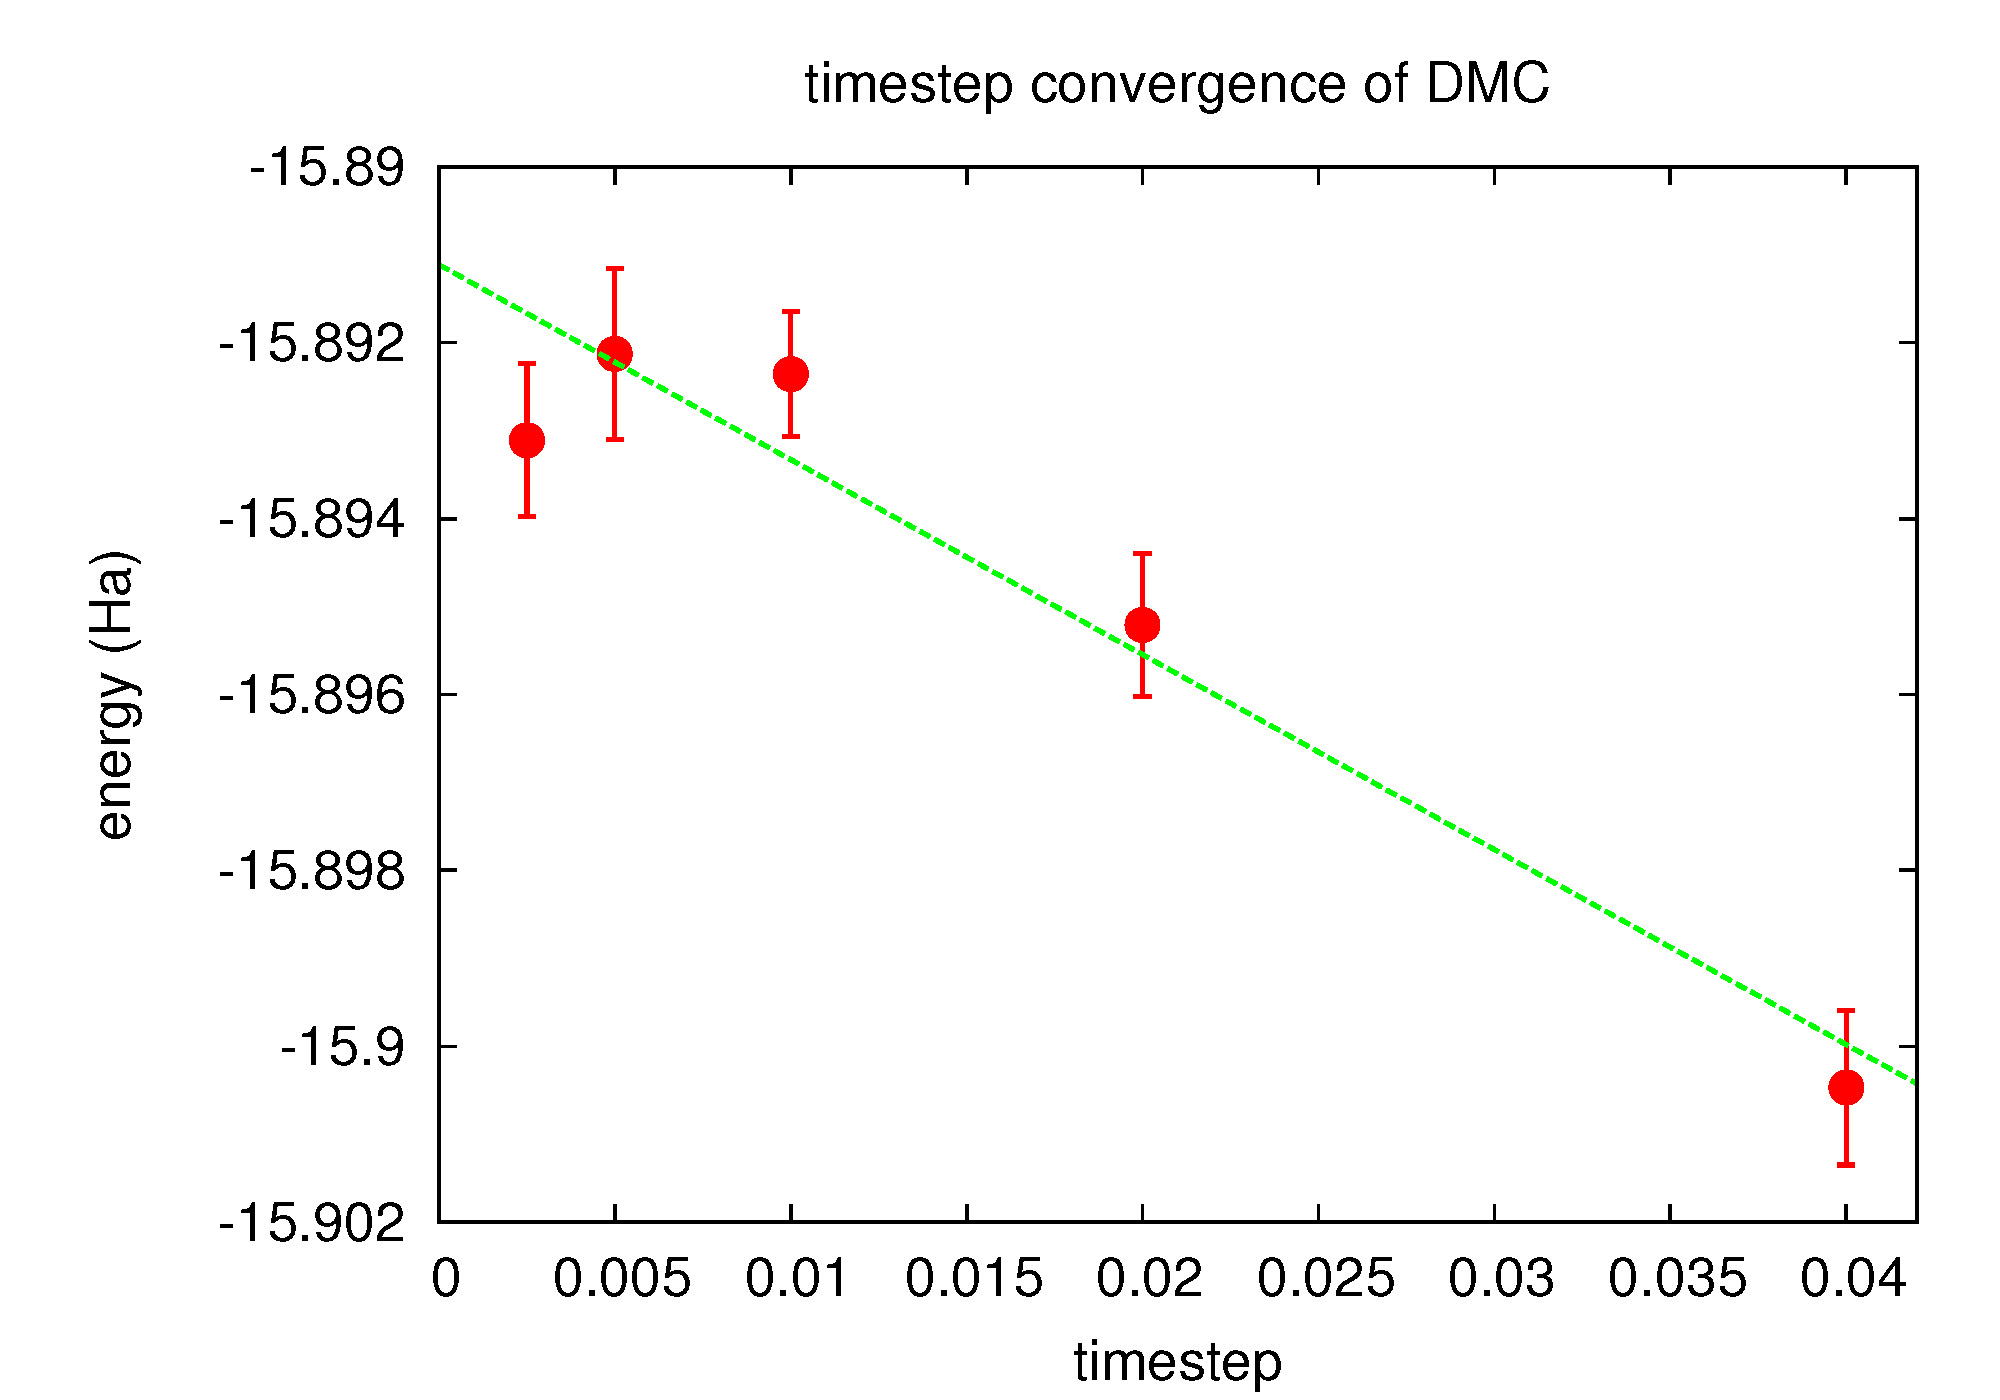
\includegraphics[trim = 0mm 0mm 0mm 0mm, clip,width=0.75\columnwidth]{./figures/lab_qmc_basics_timestep_conv.dmn}
\else
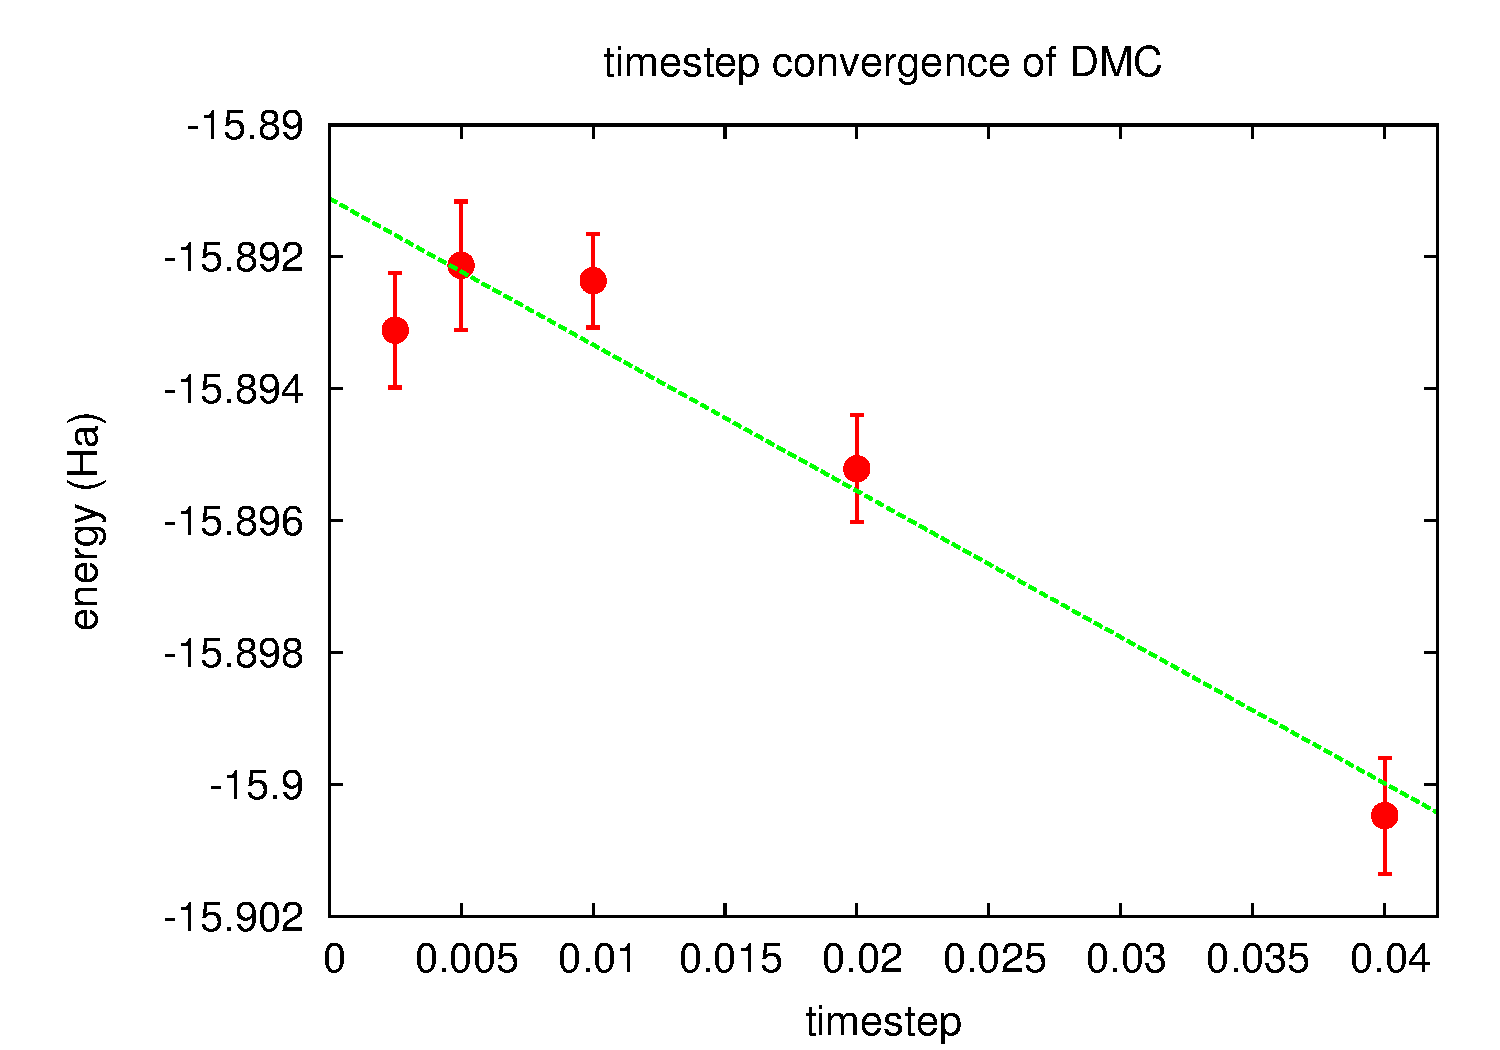
\includegraphics[trim = 0mm 0mm 0mm 0mm, clip,width=0.75\columnwidth]{./figures/lab_qmc_basics_timestep_conv.pdf}
\fi
\end{center}
\caption{Linear fit to DMC timestep data from \texttt{PlotTstepConv.pl}.}
\label{fig:timestep_conv}
\end{figure}


\vspace{1cm}
\begin{flushleft}
\textbf{\underline{Questions and Exercises}}
\end{flushleft}
\begin{enumerate}
  \item{What is the $\tau\rightarrow 0$ extrapolated value for the total energy?}
  \item{What is the maximum timestep you should use if you want to calculate the total energy to an accuracy of $0.05$ eV?  For convenience, $1~\textrm{Ha}=27.2113846~\textrm{eV}$.}
  \item{What is the acceptance ratio for this (bias$<0.05$ eV) run?  Does it follow the rule of thumb for sensible DMC (acceptance ratio $>99$\%) ?}
  \item{Check the fluctuations in the walker population (\verb|qmca -t -q nw O.q0.dmc*dmc.dat --noac|).  Does the population seem to be stable?}
  \item{(Optional) Study population control bias for the oxygen atom.  Select a few population sizes \labsw{}{(use multiples of 512 to fit cleanly on a single Vesta partition)}.  Copy \texttt{O.q0.dmc.in.xml} to a new file and remove all but one DMC run (select a single timestep).  Make one copy of the new file for each population, set ``\texttt{samples}'', and choose a unique \texttt{id} in \texttt{<project/>}.  \labsw{}{Run one job at a time to avoid crowding the lab allocation.}  Use \texttt{qmca} to study the dependence of the DMC total energy on the walker population.  How large is the bias compared to timestep error?  What bias is incurred by following the ``rule of thumb'' of a couple thousand walkers?  Will population control bias generally be an issue for production runs on modern parallel machines?}
\end{enumerate}


\section{DMC timestep extrapolation II: O atom ionization potential}
In this section, we will repeat the calculations of the prior two sections (optimization, timestep extrapolation) for the $+1$ charge state of the oxygen atom.  Comparing the resulting 1st ionization potential (IP) with experimental data will complete our first test of the BFD oxygen pseudopotential.  In actual practice, higher IP's could also be tested prior to performing production runs.

Obtaining the timestep extrapolated DMC total energy for ionized oxygen should take much less (human) time than for the neutral case.  For convenience, the necessary steps are briefly summarized below.
\begin{enumerate}
  \item{Obtain DFT orbitals with Quantum ESPRESSO}
  \begin{enumerate}
    \item{Copy the DFT input (\texttt{O.q0.dft.in}) to \texttt{O.q1.dft.in}}
    \item{Edit \texttt{O.q1.dft.in} to match the +1 charge state of the oxygen atom}
    \begin{verbatim}
     ...
     prefix            = 'O.q1'
     ...
     tot_charge        = 1
     tot_magnetization = 3
     ...
    \end{verbatim}
    \item{Perform the DFT run: \ifws\verb|mpirun -np 4 pw.x -input O.q1.dft.in >&O.q1.dft.out&|\else\verb|jobrun_vesta pw.x O.q1.dft.in|\fi}
  \end{enumerate}

  \item{Convert the orbitals to ESHDF format}
  \begin{enumerate}
    \item{Copy the pw2qmcpack input (\texttt{O.q0.p2q.in}) to \texttt{O.q1.p2q.in}}
    \item{Edit \texttt{O.q1.p2q.in} to match the file prefix used in DFT}
    \begin{verbatim}
     ...
     prefix = 'O.q1'
     ...
    \end{verbatim}
    \item{Perform the orbital conversion run: \ifws\verb|mpirun -np 1 pw2qmcpack.x<O.q1.p2q.in>&O.q1.p2q.out&|\else\verb|jobrun_vesta pw2qmcpack.x O.q1.p2q.in|\fi}
  \end{enumerate}

  \item{Optimize the Jastrow factor with QMCPACK}
  \begin{enumerate}
    \item{Copy the optimization input (\texttt{O.q0.opt.in.xml}) to \texttt{O.q1.opt.in.xml}}
    \item{Edit \texttt{O.q1.opt.in.xml} to match the file prefix used in DFT}
    \begin{lstlisting}[language=xml]
     ...
     <project id="O.q1.opt" series="0">
     ...
     <include href="O.q1.ptcl.xml"/>
     ...
     <include href="O.q1.wfs.xml"/>
     ...
    \end{lstlisting}
    \item{Edit the particle XML file (O.q1.ptcl.xml) to have open boundary conditions}
    \begin{lstlisting}[language=xml]
      <parameter name="bconds">
        n n n 
      </parameter>
    \end{lstlisting}
    \item{Add cutoffs to the Jastrow factors in the wavefunction XML file (O.q1.wfs.xml)}
    \begin{lstlisting}[language=xml]
      ...
      <correlation speciesA="u" speciesB="u" size="8" rcut="10.0">
      ...
      <correlation speciesA="u" speciesB="d" size="8" rcut="10.0">
      ...
      <correlation elementType="O" size="8" rcut="5.0">
      ...
    \end{lstlisting}
    \item{Perform the Jastrow optimization run: \ifws\verb|mpirun -np 4 qmcpack O.q1.opt.in.xml >&O.q1.opt.out&|\else\verb|jobrun_vesta qmcpack O.q1.opt.in.xml|\fi}
    \item{Identify the optimal set of parameters with \texttt{qmca} (\verb|[your opt.xml]|).}
  \end{enumerate}

  \item{DMC timestep study with QMCPACK}
  \begin{enumerate}
    \item{Copy the DMC input (\texttt{O.q0.dmc.in.xml}) to \texttt{O.q1.dmc.in.xml}}
    \item{Edit \texttt{O.q1.dmc.in.xml} to use the DFT prefix and the optimal Jastrow}
    \begin{lstlisting}[language=xml]
     ...
     <project id="O.q1.dmc" series="0">
     ...
     <include href="O.q1.ptcl.xml"/>
     ...
     <include href="[your opt.xml]"/>
     ...
    \end{lstlisting}
    \item{Perform the DMC run: \ifws\verb|mpirun -np 4 qmcpack O.q1.dmc.in.xml >&O.q1.dmc.out&|\else\verb|jobrun_vesta qmcpack O.q1.dmc.in.xml|\fi}
    \item{Obtain the DMC total energy extrapolated to zero timestep with \texttt{PlotTstepConv.pl}.}
  \end{enumerate}
\end{enumerate}
The process listed above, which excludes additional steps for orbital generation and conversion, can become tedious to perform by hand in production settings where many calculations are often required.  For this reason automation tools are introduced for calculations involving the oxygen dimer in section \ref{sec:dimer_automation} of the lab.  

\vspace{1cm}
\begin{flushleft}
\textbf{\underline{Questions and Exercises}}
\end{flushleft}
\begin{enumerate}
  \item{What is the $\tau\rightarrow 0$ extrapolated DMC value for the 1st ionization potential of oxygen?}
  \item{How does the extrapolated value compare to the experimental IP?  Go to\newline \href{http://physics.nist.gov/PhysRefData/ASD/ionEnergy.html}{http://physics.nist.gov/PhysRefData/ASD/ionEnergy.html} and enter ``\texttt{O I}'' in the box labeled ``\texttt{Spectra}'' and click on the ``\texttt{Retrieve Data}'' button.  
%For comparison the LDA value is $12.25$ eV.
}
  \item{What can we conclude about the accuracy of the pseudopotential?  What factors complicate this assessment?}
  \item{Explore the sensitivity of the IP to the choice of timestep.  Type ``\verb|./ip_conv.py|'' to view three timestep extrapolation plots: two for the $q=0,1$ total energies and one for the IP.  Is the IP more, less, or similarly sensitive to timestep than the total energy?}
  \item{What is the maximum timestep you should use if you want to calculate the ionization potential to an accuracy of $0.05$ eV?  What factor of cpu time is saved by assessing timestep convergence on the IP (a total energy difference) vs. a single total energy?}
  \item{Are the acceptance ratio and population fluctuations reasonable for the $q=1$ calculations?}
\end{enumerate}




\section{DMC workflow automation with Nexus}
Production QMC projects are often composed of many similar workflows.  The simplest of these is a single DMC calculation involving four different compute jobs:
\begin{enumerate}
  \item{Orbital generation via Quantum ESPRESSO or GAMESS.}
  \item{Conversion of orbital data via \texttt{pw2qmcpack.x} or \texttt{convert4qmc}.}
  \item{Optimization of Jastrow factors via QMCPACK.}
  \item{DMC calculation via QMCPACK.}
\end{enumerate}
Simulation workflows quickly become more complex with increasing costs in terms of human time for the researcher.  Automation tools can decrease both human time and error if used well.

The set of automation tools we will be using is known as Nexus \cite{Krogel2016nexus}, which is distributed with QMCPACK.  Nexus is capable of generating input files, submitting and monitoring compute jobs, passing data between simulations (such as relaxed structures, orbital files, optimized Jastrow parameters, etc.), and data analysis.  The user interface to Nexus is through a set of functions defined in the Python programming language.  User scripts that execute simple workflows resemble input files and do not require programming experience.  More complex workflows require only basic programming constructs (\emph{e.g.} for loops and if statements).  Nexus input files/scripts should be easier to navigate than QMCPACK input files and more efficient than submitting all the jobs by hand.

Nexus is driven by simple user-defined scripts that resemble keyword-driven input files.  An example Nexus input file that performs a single VMC calculation (with pre-generated orbitals) is shown below.  Take a moment to read it over and especially note the comments (prefixed with ``\texttt{\#}'') explaining most of the contents.  If the input syntax is unclear you may want to consult portions of appendix \ref{app:python_basics}, which gives a condensed summary of Python constructs.  An additional example and details about the inner workings of Nexus can be found in the reference publication \cite{Krogel2016nexus}. 

%For more information about the functionality and effective use of Nexus, consult \texttt{docs/Nexus.pdf}.  

%More information can be found in the user guide distributed with QMCPACK, although examples in this lab series and \texttt{Nexus.pdf} are more up to date (if \texttt{qmcpack} is the location of your QMCPACK distribution, the user guide can be found at \texttt{qmcpack/nexus/documentation/nexus\_user\_guide.pdf}).

\ifws
\begin{lstlisting}[language=Python]
#! /usr/bin/env python

# import Nexus functions
from nexus import settings,job,get_machine,run_project 
from nexus import generate_physical_system
from nexus import generate_qmcpack,vmc

settings(                             # Nexus settings
    pseudo_dir    = './pseudopotentials', # location of PP files
    runs          = '',                   # root directory for simulations
    results       = '',                   # root directory for simulation results
    status_only   = 0,                    # show simulation status, then exit
    generate_only = 0,                    # generate input files, then exit
    sleep         = 3,                    # seconds between checks on sim. progress
    machine       = 'ws4',                # workstation with 4 cores
    ) 

qmcjob = job(                         # specify job parameters
    cores   = 4,                          # use 4 MPI tasks
    threads = 1,                          # 1 OpenMP thread per node
    app     = 'qmcpack'                   # use QMCPACK executable (assumed in PATH)
    )

qmc_calcs = [                         # list QMC calculation methods
    vmc(                                  #   VMC
        walkers     =   1,                #     1 walker
        warmupsteps =  50,                #    50 MC steps for warmup
        blocks      = 200,                #   200 blocks
        steps       =  10,                #    10 steps per block
        timestep    =  .4                 #   0.4 1/Ha timestep
        )]

dimer = generate_physical_system(     # make a dimer system
    type       = 'dimer',                 # system type is dimer
    dimer      = ('O','O'),               # dimer is two oxygen atoms
    separation = 1.2074,                  # separated by 1.2074 Angstrom
    Lbox       = 15.0,                    # simulation box is 15 Angstrom 
    units      = 'A',                     # Angstrom is dist. unit
    net_spin   = 2,                       # nup-ndown is 2
    O          = 6                        # pseudo-oxygen has 6 valence el.
    )

qmc = generate_qmcpack(                # make a qmcpack simulation 
    identifier   = 'example',             # prefix files with 'example'
    path         = 'scale_1.0',           # run in ./scale_1.0 directory
    system       = dimer,                 # run the dimer system
    job          = qmcjob,                # set job parameters
    input_type   = 'basic',               # basic qmcpack inputs given below    
    pseudos      = ['O.BFD.xml'],         # list of PP's to use
    orbitals_h5  = 'O2.pwscf.h5',         # file with orbitals from DFT
    bconds       = 'nnn',                 # open boundary conditions
    jastrows     = [],                    # no jastrow factors
    calculations = qmc_calcs              # QMC calculations to perform
    )
                       
run_project(qmc)                       # write input file and submit job
\end{lstlisting}

\else

\begin{lstlisting}[language=Python]
#! /usr/bin/env python

# import Nexus functions
from nexus import settings,job,get_machine,run_project 
from nexus import generate_physical_system
from nexus import generate_qmcpack,vmc

settings(                             # Nexus settings
    pseudo_dir    = './pseudopotentials', # location of PP files
    runs          = '',                   # root directory for simulations
    results       = '',                   # root directory for simulation results
    status_only   = 0,                    # show simulation status, then exit
    generate_only = 0,                    # generate input files, then exit
    sleep         = 3,                    # seconds between checks on sim. progress
    machine       = 'vesta',              # name of local machine
    account       = 'QMCPACK-Training'    # charge account for cpu time
    ) 

vesta = get_machine('vesta')          # allow max of one job at a time (lab only)
vesta.queue_size = 1

qmcjob = job(                         # specify job parameters
    nodes   = 32,                         # use 32 Vesta nodes
    threads = 16,                         # 16 OpenMP threads per node (32 MPI tasks)
    hours   = 1,                          # wallclock limit of 1 hour
                                          # use QMCPACK executable
    app     = '/soft/applications/qmcpack/Binaries/qmcpack'
    )

qmc_calcs = [                         # list QMC calculation methods
    vmc(                                  #   VMC
        walkers     =   1,                #     1 walker
        warmupsteps =  50,                #    50 MC steps for warmup
        blocks      = 200,                #   200 blocks
        steps       =  10,                #    10 steps per block
        timestep    =  .4                 #   0.4 1/Ha timestep
        )]

dimer = generate_physical_system(     # make a dimer system
    type       = 'dimer',                 # system type is dimer
    dimer      = ('O','O'),               # dimer is two oxygen atoms
    separation = 1.2074,                  # separated by 1.2074 Angstrom
    Lbox       = 15.0,                    # simulation box is 15 Angstrom 
    units      = 'A',                     # Angstrom is dist. unit
    net_spin   = 2,                       # nup-ndown is 2
    O          = 6                        # pseudo-oxygen has 6 valence el.
    )

qmc = generate_qmcpack(                # make a qmcpack simulation 
    identifier   = 'example',             # prefix files with 'example'
    path         = 'scale_1.0',           # run in ./scale_1.0 directory
    system       = dimer,                 # run the dimer system
    job          = qmcjob,                # set job parameters
    input_type   = 'basic',               # basic qmcpack inputs given below    
    pseudos      = ['O.BFD.xml'],         # list of PP's to use
    orbitals_h5  = 'O2.pwscf.h5',         # file with orbitals from DFT
    bconds       = 'nnn',                 # open boundary conditions
    jastrows     = [],                    # no jastrow factors
    calculations = qmc_calcs              # QMC calculations to perform
    )
                       
run_project(qmc)                       # write input file and submit job
\end{lstlisting}
\fi





\section{Automated binding curve of the oxygen dimer}
\label{sec:dimer_automation}
In this section we will use Nexus to calculate the DMC total energy of the oxygen dimer over a series of bond lengths.  The equilibrium bond length and binding energy of the dimer will be determined by performing a polynomial fit to the data (Morse potential fits should be preferred in production tests).  Comparing these values with corresponding experimental data provides a second test of the BFD pseudopotential for oxygen.

Enter the \texttt{oxygen\_dimer} directory.  Copy your BFD pseudopotential from the atom runs into \texttt{oxygen\_dimer/pseudopotentials} (be sure to move both files: \texttt{.upf} and \texttt{.xml}).  Open \texttt{O\_dimer.py} with a text editor.  The overall format is similar to the example file shown in the last section.  
%The header material, including Nexus imports, settings, and the job parameters for QMC are identical.  
The main difference is that a full workflow of runs (DFT orbital generation, orbital conversion, optimization and DMC) are being performed rather than a single VMC run.  


%Following the job parameters, inputs for the optimization method are given.  The keywords should all be familiar from the QMCPACK XML input files you used previously:
%\begin{lstlisting}
%linopt1 = linear(
%    energy               = 0.0,
%    unreweightedvariance = 1.0,
%    reweightedvariance   = 0.0,
%    timestep             = 0.4,
%    samples              = 10240, 
%    warmupsteps          = 50,
%    blocks               = 200,
%    substeps             = 1,
%    nonlocalpp           = True,
%    usebuffer            = True,
%    walkers              = 1,
%    minwalkers           = 0.5,
%    maxweight            = 1e9,
%    usedrift             = True,
%    minmethod            = 'quartic',
%    beta                 = 0.025,
%    exp0                 = -16,
%    bigchange            = 15.0,
%    alloweddifference    = 1e-4,
%    stepsize             = 0.2,
%    stabilizerscale      = 1.0,
%    nstabilizers         = 3
%    )
%\end{lstlisting}
%
%%\hide{
%\noindent
%Requesting multiple loop's with different numbers of samples is more compact than in XML:
%\begin{lstlisting}
%linopt1 = ...
%
%linopt2 = linopt1.copy()  
%linopt2.samples = 61440 # opt w/ 61440 samples
%
%opt_calcs = [loop(max=4,qmc=linopt1), # loops over opt's
%             loop(max=8,qmc=linopt2)]
%\end{lstlisting}
%%}
%
%\noindent
%The VMC/DMC method inputs should also look familiar:
%\begin{lstlisting}
%qmc_calcs = [
%    vmc(
%        walkers     =   1,
%        warmupsteps =  30,
%        blocks      =  20,
%        steps       =  10,
%        substeps    =   2,
%        timestep    =  .4,
%        samples     = 2048
%        ),
%    dmc(
%        warmupsteps   = 100, 
%        blocks        = 400,
%        steps         =  32,
%        timestep      = 0.01,
%        nonlocalmoves = True
%        )
%    ]
%\end{lstlisting}


As in the example in the last section, the oxygen dimer is generated with the \texttt{generate\_physical\_system} function:
\begin{lstlisting}
dimer = generate_physical_system(
    type       = 'dimer',
    dimer      = ('O','O'),
    separation = 1.2074*scale,
    Lbox       = 10.0,
    units      = 'A',
    net_spin   = 2,
    O          = 6
    )
\end{lstlisting}
\noindent
Similar syntax can be used to generate crystal structures or to specify systems with arbitrary atomic configurations and simulation cells.  Notice that a ``\texttt{scale}'' variable has been introduced to stretch or compress the dimer.  

Next, objects representing a Quantum ESPRESSO (PWSCF) run and subsequent orbital conversion step are constructed with respective \texttt{generate\_*} functions:
\begin{lstlisting}
dft = generate_pwscf(
    identifier   = 'dft',
    ...
    input_dft    = 'lda',
    ...
    )
sims.append(dft)

# describe orbital conversion run                                                                    
p2q = generate_pw2qmcpack(
    identifier   = 'p2q',
    ...
    dependencies = (dft,'orbitals'),
    )
sims.append(p2q)
\end{lstlisting}
Note the \texttt{dependencies} keyword.  This keyword is used to construct workflows out of otherwise separate runs.  In this case, the dependency indicates that the orbital conversion run must wait for the DFT to finish prior to starting.

Objects representing QMCPACK simulations are then constructed with the \texttt{generate\_qmcpack} function:
\begin{lstlisting}
opt = generate_qmcpack(
    identifier   = 'opt',
    ...
    jastrows     = [('J1','bspline',8,5.0), 
                    ('J2','bspline',8,10.0)],
    calculations = [
        loop(max=12,
             qmc=linear(
                energy               = 0.0,
                unreweightedvariance = 1.0,
                reweightedvariance   = 0.0,
                timestep             = 0.3,
                samples              = 61440,
                warmupsteps          = 50,
                blocks               = 200,
                substeps             = 1,
                nonlocalpp           = True,
                usebuffer            = True,
                walkers              = 1,
                minwalkers           = 0.5,
                maxweight            = 1e9,
                usedrift             = False,
                minmethod            = 'quartic',
                beta                 = 0.025,
                exp0                 = -16,
                bigchange            = 15.0,
                alloweddifference    = 1e-4,
                stepsize             = 0.2,
                stabilizerscale      = 1.0,
                nstabilizers         = 3,
                )
             )
        ],
    dependencies = (p2q,'orbitals'),
    )
sims.append(opt)

qmc = generate_qmcpack(
    identifier   = 'qmc',
    ...
    jastrows     = [],            
    calculations = [
        vmc(
            walkers     =   1,
            warmupsteps =  30,
            blocks      =  20,
            steps       =  10,
            substeps    =   2,
            timestep    =  .4,
            samples     = 2048
            ),
        dmc(
            warmupsteps   = 100,
            blocks        = 400,
            steps         =  32,
            timestep      = 0.01,
            nonlocalmoves = True,
            )
        ],
    dependencies = [(p2q,'orbitals'),(opt,'jastrow')],
    )
sims.append(qmc)
\end{lstlisting}
\noindent
Shared details such as the run directory, job, pseudopotentials, and orbital file have been omitted (\texttt{...}).  The ``\texttt{opt}'' run will optimize a 1-body B-spline Jastrow with 8 knots having a cutoff of 5.0 Bohr and a B-spline Jastrow (for up-up and up-down correlations) with 8 knots and cutoffs of 10.0 Bohr.  The Jastrow list for the DMC run is empty and the usage of \texttt{dependencies} above indicates that the DMC run depends on the optimization run for the Jastrow factor.  Nexus will submit the ``\texttt{opt}'' run first and upon completion it will scan the output, select the optimal set of parameters, pass the Jastrow information to the ``\texttt{qmc}'' run and then submit the DMC job.  Independent job workflows are submitted in parallel when permitted \labsw{}{(we have explicitly limited this for this lab by setting \texttt{queue\_size=2} for Vesta)}.  No input files are written or job submissions made until the ``\texttt{run\_project}'' function is reached:
\begin{lstlisting}
run_project(sims)
\end{lstlisting}
\noindent
All of the simulations objects have been collected into a list (\texttt{sims}) for submission.

As written, \texttt{O\_dimer.py} will only perform calculations at the equilibrium separation distance of 1.2074 Angstrom, since the list of scaling factors (representing stretching or compressing the dimer) only contains one value (\texttt{scales = [1.00]}).  Modify the file now to perform DMC calculations across a range of separation distances with each DMC run using the Jastrow factor optimized at the equilibrium separation distance.  Specifically, you will want to change the list of scaling factors to include both compression (\texttt{scale<1.0}) and stretch (\texttt{scale>1.0}): 
\begin{lstlisting}
scales = [1.00,0.90,0.95,1.05,1.10]
\end{lstlisting}
\noindent
Note that ``\texttt{1.00}'' is left in front because we are going to optimize the Jastrow factor first at the equilibrium separation and reuse this Jastrow factor for all other separation distances.  This procedure is used because it can reduce variations in localization errors (due to pseudopotentials in DMC) along the binding curve. 

Change the ``\texttt{status\_only}'' parameter in the ``\texttt{settings}'' function to \texttt{1} and type ``./O\_dimer.py'' at the command line.  This will print the status of all simulations:
\begin{shade}
Project starting 
  checking for file collisions 
  loading cascade images 
    cascade 0 checking in 
    cascade 10 checking in 
    cascade 4 checking in 
    cascade 13 checking in 
    cascade 7 checking in 
  checking cascade dependencies 
    all simulation dependencies satisfied 
  
  cascade status 
    setup, sent_files, submitted, finished, got_output, analyzed 
    000000  dft     ./scale_1.0 
    000000  p2q     ./scale_1.0 
    000000  opt     ./scale_1.0 
    000000  qmc     ./scale_1.0 
    000000  dft     ./scale_0.9 
    000000  p2q     ./scale_0.9 
    000000  qmc     ./scale_0.9 
    000000  dft     ./scale_0.95 
    000000  p2q     ./scale_0.95 
    000000  qmc     ./scale_0.95 
    000000  dft     ./scale_1.05 
    000000  p2q     ./scale_1.05 
    000000  qmc     ./scale_1.05 
    000000  dft     ./scale_1.1 
    000000  p2q     ./scale_1.1 
    000000  qmc     ./scale_1.1 
    setup, sent_files, submitted, finished, got_output, analyzed 
\end{shade}
\noindent
In this case, five simulation ``cascades'' (workflows) have been identified, each one starting and ending with ``\texttt{dft}'' and ``\texttt{qmc}'' runs, respectively.  The six status flags (\texttt{setup}, \texttt{sent\_files}, \texttt{submitted}, \texttt{finished}, \texttt{got\_output}, \texttt{analyzed}) each show \texttt{0}, indicating that no work has been done yet.  

Now change ``\texttt{status\_only}'' back to \texttt{0}, set ``\texttt{generate\_only}'' to \texttt{1}, and run \texttt{O\_dimer.py} again.  This will perform a dry-run of all simulations.  The dry-run should finish in about 20 seconds:
\ifws
\begin{shade}
Project starting 
  checking for file collisions 
  loading cascade images 
    cascade 0 checking in 
    cascade 10 checking in 
    cascade 4 checking in 
    cascade 13 checking in 
    cascade 7 checking in 
  checking cascade dependencies 
    all simulation dependencies satisfied 
  
  starting runs:
  ~~~~~~~~~~~~~~~~~~~~~~~~~~~~~~ 
  poll 0  memory 91.03 MB 
    Entering ./scale_1.0 0 
      writing input files  0 dft 
    Entering ./scale_1.0 0 
      sending required files  0 dft 
      submitting job  0 dft 
  ...
  poll 1  memory 91.10 MB 
  ...
    Entering ./scale_1.0 0 
      Would have executed:  
        export OMP_NUM_THREADS=1
        mpirun -np 4 pw.x -input dft.in 

  poll 2  memory 91.10 MB 
    Entering ./scale_1.0 0 
      copying results  0 dft 
    Entering ./scale_1.0 0 
      analyzing  0 dft 
  ...
  poll 3  memory 91.10 MB 
    Entering ./scale_1.0 1 
      writing input files  1 p2q 
    Entering ./scale_1.0 1 
      sending required files  1 p2q 
      submitting job  1 p2q 
  ...
    Entering ./scale_1.0 1 
      Would have executed:  
        export OMP_NUM_THREADS=1
        mpirun -np 1 pw2qmcpack.x<p2q.in 

  poll 4  memory 91.10 MB 
    Entering ./scale_1.0 1 
      copying results  1 p2q 
    Entering ./scale_1.0 1 
      analyzing  1 p2q 
  ...
  poll 5  memory 91.10 MB 
    Entering ./scale_1.0 2 
      writing input files  2 opt 
    Entering ./scale_1.0 2 
      sending required files  2 opt 
      submitting job  2 opt 
  ...
    Entering ./scale_1.0 2 
      Would have executed:  
        export OMP_NUM_THREADS=1
        mpirun -np 4 qmcpack opt.in.xml 

  poll 6  memory 91.16 MB 
    Entering ./scale_1.0 2 
      copying results  2 opt 
    Entering ./scale_1.0 2 
      analyzing  2 opt 
  ...
  poll 7  memory 93.00 MB 
    Entering ./scale_1.0 3 
      writing input files  3 qmc 
    Entering ./scale_1.0 3 
      sending required files  3 qmc 
      submitting job  3 qmc 
  ...
    Entering ./scale_1.0 3 
      Would have executed:  
        export OMP_NUM_THREADS=1
        mpirun -np 4 qmcpack qmc.in.xml 
  ...
  poll 17  memory 93.06 MB 
Project finished
\end{shade}
\else
\begin{shade}
Project starting 
  checking for file collisions 
  loading cascade images 
    cascade 0 checking in 
    cascade 10 checking in 
    cascade 4 checking in 
    cascade 13 checking in 
    cascade 7 checking in 
  checking cascade dependencies 
    all simulation dependencies satisfied 
  
  starting runs:
  ~~~~~~~~~~~~~~~~~~~~~~~~~~~~~~ 
  poll 0  memory 91.03 MB 
    Entering ./scale_1.0 0 
      writing input files  0 dft 
    Entering ./scale_1.0 0 
      sending required files  0 dft 
      submitting job  0 dft 
  ...
  poll 1  memory 91.10 MB 
  ...
    Entering ./scale_1.0 1 
      Would have executed:  qsub --mode script --env BG_SHAREDMEMSIZE=32 dft.qsub.in 

  poll 2  memory 91.10 MB 
    Entering ./scale_1.0 0 
      copying results  0 dft 
    Entering ./scale_1.0 0 
      analyzing  0 dft 
  ...
  poll 3  memory 91.10 MB 
    Entering ./scale_1.0 1 
      writing input files  1 p2q 
    Entering ./scale_1.0 1 
      sending required files  1 p2q 
      submitting job  1 p2q 
  ...
    Entering ./scale_1.0 2 
      Would have executed:  qsub --mode script --env BG_SHAREDMEMSIZE=32 p2q.qsub.in 

  poll 4  memory 91.10 MB 
    Entering ./scale_1.0 1 
      copying results  1 p2q 
    Entering ./scale_1.0 1 
      analyzing  1 p2q
  ... 

  poll 5  memory 91.10 MB 
    Entering ./scale_1.0 2 
      writing input files  2 opt 
    Entering ./scale_1.0 2 
      sending required files  2 opt 
      submitting job  2 opt 
  ...
    Entering ./scale_1.0 3 
      Would have executed:  qsub --mode script --env BG_SHAREDMEMSIZE=32 opt.qsub.in 

  poll 6  memory 91.16 MB 
    Entering ./scale_1.0 2 
      copying results  2 opt 
    Entering ./scale_1.0 2 
      analyzing  2 opt 
  ...
  poll 7  memory 93.00 MB 
    Entering ./scale_1.0 3 
      writing input files  3 qmc 
    Entering ./scale_1.0 3 
      sending required files  3 qmc 
      submitting job  3 qmc 
  ...
    Entering ./scale_1.0 4 
      Would have executed:  qsub --mode script --env BG_SHAREDMEMSIZE=32 qmc.qsub.in 
  ...

  poll 17  memory 93.00 MB 
Project finished
\end{shade}
\fi

\noindent
Nexus polls the simulation status every 3 seconds and sleeps in between.  The ``scale\_*'' directories should now contain several files:
\ifws
\begin{shade}
scale_1.0
   dft.in
   O.BFD.upf
   O.BFD.xml
   opt.in.xml
   p2q.in
   pwscf_output
   qmc.in.xml
   sim_dft/
       analyzer.p
       input.p
       sim.p
   sim_opt/
       analyzer.p
       input.p
       sim.p
   sim_p2q/
       analyzer.p
       input.p
       sim.p
   sim_qmc/
       analyzer.p
       input.p
       sim.p
\end{shade}
\else
\begin{shade}
scale_1.0
   dft.in
   dft.qsub.in
   O.BFD.upf
   O.BFD.xml
   opt.in.xml
   opt.qsub.in
   p2q.in
   p2q.qsub.in
   pwscf_output
   qmc.in.xml
   qmc.qsub.in
   sim_dft/
       analyzer.p
       input.p
       sim.p
   sim_opt/
       analyzer.p
       input.p
       sim.p
   sim_p2q/
       analyzer.p
       input.p
       sim.p
   sim_qmc/
       analyzer.p
       input.p
       sim.p
\end{shade}
\fi
\noindent
Take a minute to inspect the generated input (\texttt{dft.in}, \texttt{p2q.in}, \texttt{opt.in.xml}, \texttt{qmc.in.xml}) \labsw{}{and submission (\texttt{dft.qsub.in}, \texttt{p2q.qsub.in}, \texttt{opt.qsub.in}, \texttt{qmc.qsub.in})} files.  The pseudopotential files (\texttt{O.BFD.upf} and \texttt{O.BFD.xml}) have been copied into each local directory. Four additional directories have been created: \texttt{sim\_dft},  \texttt{sim\_p2q}, \texttt{sim\_opt} and \texttt{sim\_qmc}.  The \texttt{sim.p} files in each directory contain the current status of each simulation.  If you run \texttt{O\_dimer.py} again, it should not attempt to rerun any of the simulations:   
\begin{shade}
Project starting 
  checking for file collisions 
  loading cascade images 
    cascade 0 checking in 
    cascade 10 checking in 
    cascade 4 checking in 
    cascade 13 checking in 
    cascade 7 checking in 
  checking cascade dependencies 
    all simulation dependencies satisfied 
  
  starting runs:
  ~~~~~~~~~~~~~~~~~~~~~~~~~~~~~~ 
  poll 0  memory 64.25 MB 
Project finished
\end{shade}
\noindent
This way one can continue to add to the \texttt{O\_dimer.py} file (\emph{e.g.} adding more separation distances) without worrying about duplicate job submissions.

Let's actually submit the jobs in the dimer workflow now.  Reset the state of the simulations by removing the \texttt{sim.p} files (``\texttt{rm ./scale*/sim*/sim.p}''), set ``\texttt{generate\_only}'' to \texttt{0}, and rerun \texttt{O\_dimer.py}.  It should take about 20 minutes for all the jobs to complete.  You may wish to open another terminal to monitor the progress of the individual jobs while the current terminal runs \texttt{O\_dimer.py} in the foreground.  You can begin the first exercise below once the optimization job completes.

\vspace{3cm}
\begin{flushleft}
\textbf{\underline{Questions and Exercises}}
\end{flushleft}
\begin{enumerate}
  \item{Evaluate the quality of the optimization at \texttt{scale=1.0} using the \texttt{qmca} tool.  Did the optimization succeed?  How does the variance compare with the neutral oxygen atom?  Is the wavefunction of similar quality to the atomic case?}

  \item{Evaluate the traces of the local energy and the DMC walker population for each separation distance with the \texttt{qmca} tool.  Are there any anomalies in the runs?  Is the acceptance ratio reasonable?  Is the wavefunction of similar quality across all separation distances?}

  \item{Use the \texttt{dimer\_fit.py} tool located in \texttt{oxygen\_dimer} to fit the oxygen dimer binding curve.   To get the binding energy of the dimer, we will need the DMC energy of the atom.  Before performing the fit, answer: What DMC timestep should be used for the oxygen atom results?  The tool accepts three arguments (``\verb|./dimer_fit.py P N E Eerr|''}), \texttt{P} is the prefix of the DMC input files (should be ``\texttt{qmc}'' at this point), \texttt{N} is the order of the fit (use 2 to start), \texttt{E} and \texttt{Eerr} are your DMC total energy and error bar, respectively for the oxygen atom (in eV).  A plot of the dimer data will be displayed and text output will show the DMC equilibrium bond length and binding energy as well as experimental values.  How accurately does your fit to the DMC data reproduce the experimental values?  What factors affect the accuracy of your results? 

  \item{Refit your data with a fourth-order polynomial.  How do your predictions change with a fourth-order fit?  Is a fourth-order fit appropriate for the available data?}
 
  \item{Add new ``\texttt{scale}'' values to the list in \texttt{O\_dimer.py} that interpolate between the original set (e.g. expand to \texttt{[1.00,0.90,0.925,0.95,0.975,1.025,1.05,1.075,1.10]}).  Perform the DMC calculations and redo the fits.  How accurately does your fit to the DMC data reproduce the experimental values?  Should this pseudopotential be used in production calculations?}

  \item{(Optional) Perform optimization runs at the extremal separation distances corresponding to \texttt{scale=[0.90,1.10]}}.  Are the individually optimized wavefunctions of significantly better quality than the one imported from \texttt{scale=1.00}?  Why?  What form of Jastrow factor might give an even better improvement? 
\end{enumerate}




\section{(Optional) Running your system with QMCPACK}\label{sec:your_system}
This section covers a fairly simple route to get started on QMC calculations of an arbitrary system of interest using the Nexus workflow management system to setup input files and optionally perform the runs.  The example provided in this section uses QM Espresso (PWSCF) to generate the orbitals forming the Slater determinant part of the trial wavefunction.  PWSCF is a natural choice for solid state systems and it can be used for surface/slab and molecular systems as well, albeit at the price of describing additional vacuum space with plane waves.

To start out with, you will need pseudopotentials (PP's) for each element in your system in both the UPF (PWSCF) and FSATOM/XML (QMCPACK) formats.  A good place to start is the Burkatzki-Filippi-Dolg (BFD) pseudopotential database \newline (\href{http://www.burkatzki.com/pseudos/index.2.html}{http://www.burkatzki.com/pseudos/index.2.html}), which we have already used in our study of the oxygen atom.  The database does not contain PP's for the 4th and 5th row transition metals or any of the lanthanides or actinides.  If you need a PP that is not in the BFD database, you may need to generate and test one manually (\emph{e.g.} with OPIUM, \href{http://opium.sourceforge.net/}{http://opium.sourceforge.net/}).  Otherwise, use \texttt{ppconvert} as outlined in section \ref{sec:lqb_pseudo} to obtain PP's in the formats used by PWSCF and QMCPACK.  Enter the \texttt{your\_system} lab directory and place the converted PP's in \texttt{your\_system/pseudopotentials}.

Before performing production calculations (more than just the initial setup in this section) be sure to converge the plane wave energy cutoff in PWSCF as these PP's can be rather hard, sometimes requiring cutoffs in excess of 300 Ry.  Depending on the system under study, the amount of memory required to represent the orbitals (QMCPACK uses 3D B-splines) becomes prohibitive and one may be forced to search for softer PP's.

Beyond pseudopotentials, all that is required to get started are the atomic positions and the dimensions/shape of the simulation cell.  The Nexus file \texttt{example.py} illustrates how to setup PWSCF and QMCPACK input files by providing minimal information regarding the physical system (an 8-atom cubic cell of diamond in the example).  Most of the contents should be familiar from your experience with the automated calculations of the oxygen dimer binding curve in section \ref{sec:dimer_automation} (if you've skipped ahead you may want to skim that section for relevant information).  The most important change is the expanded description of the physical system:

\begin{lstlisting}[language=Python]
# details of your physical system (diamond conventional cell below)
my_project_name = 'diamond_vmc'   # directory to perform runs
my_dft_pps      = ['C.BFD.upf']   # pwscf pseudopotentials
my_qmc_pps      = ['C.BFD.xml']   # qmcpack pseudopotentials

#  generate your system
#    units      :  'A'/'B' for Angstrom/Bohr
#    axes       :  simulation cell axes in cartesian coordinates (a1,a2,a3)
#    elem       :  list of atoms in the system
#    pos        :  corresponding atomic positions in cartesian coordinates
#    kgrid      :  Monkhorst-Pack grid
#    kshift     :  Monkhorst-Pack shift (between 0 and 0.5)
#    net_charge :  system charge in units of e
#    net_spin   :  # of up spins - # of down spins
#    C = 4      :  (pseudo) carbon has 4 valence electrons
my_system = generate_physical_system(
    units      = 'A',
    axes       = [[ 3.57000000e+00, 0.00000000e+00, 0.00000000e+00],
                  [ 0.00000000e+00, 3.57000000e+00, 0.00000000e+00],
                  [ 0.00000000e+00, 0.00000000e+00, 3.57000000e+00]],
    elem       = ['C','C','C','C','C','C','C','C'],
    pos        = [[ 0.00000000e+00, 0.00000000e+00, 0.00000000e+00],
                  [ 8.92500000e-01, 8.92500000e-01, 8.92500000e-01],
                  [ 0.00000000e+00, 1.78500000e+00, 1.78500000e+00],
                  [ 8.92500000e-01, 2.67750000e+00, 2.67750000e+00],
                  [ 1.78500000e+00, 0.00000000e+00, 1.78500000e+00],
                  [ 2.67750000e+00, 8.92500000e-01, 2.67750000e+00],
                  [ 1.78500000e+00, 1.78500000e+00, 0.00000000e+00],
                  [ 2.67750000e+00, 2.67750000e+00, 8.92500000e-01]],
    kgrid      = (1,1,1),
    kshift     = (0,0,0),
    net_charge = 0,
    net_spin   = 0,
    C          = 4       # one line like this for each atomic species
    )

my_bconds       = 'ppp'  #  ppp/nnn for periodic/open BC's in QMC
                         #  if nnn, center atoms about (a1+a2+a3)/2
\end{lstlisting}

If you have a system you would like to try with QMC, make a copy of \texttt{example.py} and fill in the relevant information about the pseudopotentials, simulation cell axes, and atomic species/positions.  Otherwise, you can proceed with \texttt{example.py} as it is.

%The other new aspects are two additional compute jobs to generate the orbitals with PWSCF and convert them into the ESHDF format with \texttt{pw2qmcpack.x}:

%\begin{lstlisting}
%# scf run to generate orbitals
%scf = generate_pwscf(
%    identifier   = 'scf',
%    path         = my_project_name,
%    job          = Job(nodes=32,hours=2,app=pwscf),
%    input_type   = 'scf',
%    system       = my_system,
%    pseudos      = my_dft_pps,
%    input_dft    = 'lda', 
%    ecut         = 200,   # PW energy cutoff in Ry
%    conv_thr     = 1e-8, 
%    mixing_beta  = .7,
%    nosym        = True,
%    wf_collect   = True
%    )
%
%# conversion step to create h5 file with orbitals
%p2q = generate_pw2qmcpack(
%    identifier   = 'p2q',
%    path         = my_project_name,
%    job          = Job(cores=1,hours=2,app=pw2qmcpack),
%    write_psir   = False,
%    dependencies = (scf,'orbitals')
%    )
%\end{lstlisting}

Set ``\texttt{generate\_only}'' to \texttt{1} and type ``\texttt{./example.py}'' or similar to generate the input files.  All files will be written to ``\texttt{./diamond\_vmc}'' (``\texttt{./[my\_project\_name]}'' if you have changed ``\texttt{my\_project\_name}'' in the file).  The input files for PWSCF, pw2qmcpack, and QMCPACK are \texttt{scf.in}, \texttt{pw2qmcpack.in}, and \texttt{vmc.in.xml}, respectively.  Take some time to inspect the generated input files.  If you have questions about the file contents, or run into issues with the generation process, feel free to consult with a lab instructor.  

If desired, you can submit the runs directly with \texttt{example.py}.  To do this, first reset the Nexus simulation record by typing ``\texttt{rm ./diamond\_vmc/sim*/sim.p}'' or similar and set ``\texttt{generate\_only}'' back to \texttt{0}.  Next rerun \texttt{example.py}  (you may want to redirect the text output).  

Alternatively the runs can be submitted by hand:
\ifws
\begin{shade}
mpirun -np 4 pw.x<scf.in>&scf.out&

(wait until JOB DONE appears in scf.out)

mpirun -np 1 pw2qmcpack.x<p2q.in>&p2q.out&
\end{shade}
\else
\begin{shade}
qsub --mode script --env BG_SHAREDMEMSIZE=32 scf.qsub.in

(wait until JOB DONE appears in scf.output)

qsub --mode script --env BG_SHAREDMEMSIZE=32 p2q.qsub.in
\end{shade}
\fi
Once the conversion process has finished the orbitals should be located in the file \newline \texttt{diamond\_vmc/pwscf\_output/pwscf.pwscf.h5}.  Open \texttt{diamond\_vmc/vmc.in.xml} and replace ``\texttt{MISSING.h5}'' with ``\texttt{./pwscf\_output/pwscf.pwscf.h5}''.  Next submit the VMC run:
\ifws
\begin{shade}
mpirun -np 4 qmcpack vmc.in.xml>&vmc.out&
\end{shade}
\else
\begin{shade}
qsub --mode script --env BG_SHAREDMEMSIZE=32 vmc.qsub.in
\end{shade}
\fi
Note: If your system is large, the above process may not complete within the time frame of this lab.  Working with a stripped down (but relevant) example is a good idea for exploratory runs.

Once the runs have finished, you may want to begin exploring Jastrow optimization and DMC for your system.  Example calculations are provided at the end of \texttt{example.py} in the commented out text.



%\section{(Optional) Revisiting the oxygen atom: 3-body Jastrow \& population control bias}

%\subsection{Optimization of 3-body Jastrow factors}

%\subsection{Investigation of DMC population control bias}




% cover basic python elsewhere in the manual?  refer to Nexus user guide or websites instead?
%\hide{

\section{Appendix A: Basic Python constructs\label{app:python_basics}}
Basic Python data types (\texttt{int}, \texttt{float}, \texttt{str}, \texttt{tuple}, \texttt{list}, \texttt{array}, \texttt{dict}, \texttt{obj}) and programming constructs (\texttt{if} statements, \texttt{for} loops, functions w/ keyword arguments) are briefly overviewed below.  All examples can be executed interactively in Python.  To do this, type ``\texttt{python}'' at the command line and paste any of the shaded text below at the ``\texttt{>>>}'' prompt.  For more information about effective use of Python, consult the detailed online documentation: \href{https://docs.python.org/2/}{https://docs.python.org/2/}.

\subsubsection{Intrinsic types: \texttt{int, float, str}}
\begin{shade}
#this is a comment
i=5                     # integer
f=3.6                   # float
s='quantum/monte/carlo' # string
n=None                  # represents "nothing"

f+=1.4                  # add-assign (-,*,/ also): 5.0
2**3                    # raise to a power: 8
str(i)                  # int to string: '5'
s+'/simulations'        # joining strings: 'quantum/monte/carlo/simulations'
'i={0}'.format(i)       # format string: 'i=5'

\end{shade}

 
\subsubsection{Container types: \texttt{tuple, list, array, dict, obj}}
\begin{shade}
from numpy import array  # get array from numpy module
from generic import obj  # get obj from Nexus' generic module 

t=('A',42,56,123.0)     # tuple

l=['B',3.14,196]        # list

a=array([1,2,3])        # array

d={'a':5,'b':6}         # dict

o=obj(a=5,b=6)          # obj

                        # printing
print t                 #  ('A', 42, 56, 123.0)
print l                 #  ['B', 3.1400000000000001, 196]
print a                 #  [1 2 3]
print d                 #  {'a': 5, 'b': 6}
print o                 #    a               = 5
                        #    b               = 6

len(t),len(l),len(a),len(d),len(o) #number of elements: (4, 3, 3, 2, 2)

t[0],l[0],a[0],d['a'],o.a  #element access: ('A', 'B', 1, 5, 5)

s = array([0,1,2,3,4])  # slices: works for tuple, list, array
s[:]                    #   array([0, 1, 2, 3, 4])
s[2:]                   #   array([2, 3, 4])
s[:2]                   #   array([0, 1])
s[1:4]                  #   array([1, 2, 3])
s[0:5:2]                #   array([0, 2, 4])

                        # list operations
l2 = list(l)            #   make independent copy
l.append(4)             #   add new element: ['B', 3.14, 196, 4]
l+[5,6,7]               #   addition: ['B', 3.14, 196, 4, 5, 6, 7]
3*[0,1]                 #   multiplication:  [0, 1, 0, 1, 0, 1]

b=array([5,6,7])        # array operations
a2 = a.copy()           #   make independent copy
a+b                     #   addition: array([ 6, 8, 10])
a+3                     #   addition: array([ 4, 5, 6])
a*b                     #   multiplication: array([ 5, 12, 21])
3*a                     #   multiplication: array([3, 6, 9])

                        # dict/obj operations
d2 = d.copy()           #   make independent copy
d['c'] = 7              #   add/assign element 
d.keys()                #   get element names: ['a', 'c', 'b']
d.values()              #   get element values: [5, 7, 6]

                        # obj-specific operations
o.c = 7                 #   add/assign element
o.set(c=7,d=8)          #   add/assign multiple elements

\end{shade}
An important feature of Python to be aware of is that assignment is most often by reference, \emph{i.e.} new values are not always created.  This point is illustrated below with an \texttt{obj} instance, but it also holds for \texttt{list}, \texttt{array}, \texttt{dict}, and others.
\begin{shade}
>>> o = obj(a=5,b=6)
>>> 
>>> p=o
>>> 
>>> p.a=7
>>> 
>>> print o
  a               = 7
  b               = 6

>>> q=o.copy()
>>> 
>>> q.a=9
>>> 
>>> print o
  a               = 7
  b               = 6
\end{shade}
\noindent
Here \texttt{p} is just another name for \texttt{o}, while \texttt{q} is a fully independent copy of it.


\subsubsection{Conditional Statements: \texttt{if/elif/else}}
\begin{shade}
a = 5
if a is None:
    print 'a is None'
elif a==4:
    print 'a is 4'
elif a<=6 and a>2:
    print 'a is in the range (2,6]'
elif a<-1 or a>26:
    print 'a is not in the range [-1,26]'
elif a!=10: 
    print 'a is not 10'
else:
    print 'a is 10'
#end if

\end{shade}
The ``\texttt{\#end if}'' is not part of Python syntax, but you will see text like this throughout Nexus for clear encapsulation.

\subsubsection{Iteration: \texttt{for}}
\begin{shade}
from generic import obj

l = [1,2,3]              
m = [4,5,6]
s = 0
for i in range(len(l)):  # loop over list indices
    s += l[i] + m[i]
#end for

print s                  # s is 21

s = 0                    
for v in l:              # loop over list elements
    s += v
#end for

print s                  # s is 6

o = obj(a=5,b=6)
s = 0
for v in o:              # loop over obj elements
    s += v
#end for

print s                  # s is 11

d = {'a':5,'b':4}
for n,v in o.iteritems():# loop over name/value pairs in obj
    d[n] += v
#end for

print d                  # d is {'a': 10, 'b': 10}

\end{shade}


\subsubsection{Functions: \texttt{def}, argument syntax}
\begin{shade}
def f(a,b,c=5):          # basic function, c has a default value
    print a,b,c
#end def f

f(1,b=2)                 # prints: 1 2 5


def f(*args,**kwargs):   # general function, returns nothing
    print args           #     args: tuple of positional arguments
    print kwargs         #   kwargs: dict of keyword arguments
#end def f

f('s',(1,2),a=3,b='t')   # 2 pos., 2 kw. args, prints:
                         #   ('s', (1, 2))
                         #   {'a': 3, 'b': 't'}

l = [0,1,2]
f(*l,a=6)                # pos. args from list, 1 kw. arg, prints:
                         #   (0, 1, 2)
                         #   {'a': 6}
o = obj(a=5,b=6)
f(*l,**o)                # pos./kw. args from list/obj, prints:
                         #   (0, 1, 2)
                         #   {'a': 5, 'b': 6}

f(                       # indented kw. args, prints
    blocks   = 200,      #   () 
    steps    = 10,       #   {'steps': 10, 'blocks': 200, 'timestep': 0.01}
    timestep = 0.01
    )

o = obj(                 # obj w/ indented kw. args
    blocks   = 100,
    steps    =  5,
    timestep = 0.02
    )

f(**o)                   # kw. args from obj, prints:
                         #   ()
                         #   {'timestep': 0.02, 'blocks': 100, 'steps': 5}
\end{shade}

%}
